\subsection{Programming setup}
Data augmentation using deep learing is a highly complicated process, so choosing the right tooling plays a crucial role in it. Lack of knowledge about modern technologies that help with programming environment setup may lead to many hours of additional time spent on the project that are not specifically related to the core analysis. In order to reduce the time spent on configuration errors, modern state-of-the-art technologies were employed to mitigate this issue.  

\paragraph{Git}\mbox{}\\
\indent Git is a software code versioning system created in 2005. It allows the user to have a local copy of the project code and propose changes to the main copy stored on the remote server, such as Github. Thanks to this tool, collaboration between different programmers is possible. Additionally, unsuccessful attempts or flaws in the implementation may be reverted to the original state.
\paragraph{Github}\mbox{}\\
\indent Enables the user to store git repository on the remote server. The project code is stored in the Github repository.
\paragraph{Data Science project structure}\mbox{}\\
\indent Data Science projects like this often take different forms. Lack of standarization - where and what is stored, may lead to decrease of programmers' productivity over time. Data Science cookie-cutter authors came in the front of this issue. They created a standardized Data Science project structure that can be used to implement a variety of Machine Learning models. 
It has the following form:

\lstinputlisting[basicstyle=\ttfamily\tiny]{detailed_engineering/folder_structure.txt}


The existing project was inspired by the template.
\paragraph{VSCode Remote SSH}\mbox{}\\
\indent Working on a remote computer can be a difficult task to handle. Remote environments often lack the tools that make a programmer effective. Especially a code editor and extensions that the programmer is used to work with and which make a programmer effective in writing code and detecting bugs. VSCode Remote SSH enables a programmer that uses Visual Studio Code to connect to a remote machine with the current editor, so it is almost indistinguishable from the experience of working on a local machine. This way no time was spent on remote code editor setup and extensions installation and configuration. 

\paragraph{Devbox}\mbox{}\\
\indent Remote computers often have their administrators. Almost always they are only ones who are in the super-users' group called "sudoers" in a Linux environment. It helps them keep the machine secure, but also makes them only persons who are able to install additional software, which is later available for everyone. On the other hand, it raises an issue of additional package installation - like specific Python versions and CLI's (Command Line Interfaces) that are required by a project or make a programmer productive.  
To mitigate this issue, a programmer can install software only for himself. However, with the standard Debian/Ubnutu package installer, "apt", it is hard to employ this strategy since many commands still require sudo access. 

Devbox makes it possible to create an environment per project and specify the exact versions of software that should be installed. It can be integrated with Git and Github to make it possible for other programmers to reproduce execalty the same enviornment on their computers. 

Devbox uses the "Nix" package installer under the hood. It is currently the biggest package manager that exists in the Unix landscape. It allows to install most of the open source software that has been ever created. Unfortunatelly, it uses a language that has been specifically created for it. Devbox make it possible to define programs that should be installed in a json file with a specific structure and pin a specific version of the software. Then it creates a lock file in which exact versions for each platform with hashes of the programs are stored. It makes it possible to fully recreate the programming environment created on one computer on another.

CLIs, drivers, versions pinned and managed by the nix package manager.
When it comes to programming environment setup, 

\paragraph{Direnv}\mbox{}\\
\indent When it comes to working with programming projects, the programmer has to switch between them. It requires a Python programmer to change the Python environment to the right one that consists of everything that the project requires to run. Direnv automatically activates the right environment when a directory of the project is entered, so the programmer does not have to do it manually and remember about it.

In the project - Devbox environment and Python environment are automatically enabled when a programmer enters the project directory (and has direnv installed).
\paragraph{Python}\mbox{}\\
\indent Numerous programming languages such as Matlab, Julia, and Elixir support the development of deep learning projects. However, Python stands out as the primary language for most research and advancements in Artificial Intelligence. Therefore, it was the natural choice for this project.
\paragraph{Rye}\mbox{}\\
\indent Almost every Python project nowadays uses external libraries written by other programmers. It makes the programmer not reinvent the wheel again and dramatically reduces the project implementation time. However, it raises the issue of external package version management. To tackle this issue, Python programmers came up with the'requirements.txt' file that should include all external, non-standard, dependencies that the project requires in order to make the environment reproducible on the other computer. In addition, they introduced the `pip` package manager that allows them to be installed. 
Rye is a more modern solution to this problem. It enables the user to create a Python package from the existing project, define external dependencies with their exact versions, and create a Python virtual environment. 

What is more - it makes it possible to use a modern replacement for the `pip` package manager - uv. UV is a modern package installer written in Rust that is in some cases even 100 times faster in comparison to its predecessor.  
\paragraph{Pytorch}\mbox{}\\
\indent Pytorch is a Deep Learning framework for Python programmers. It makes it possible to create neural networks and train them on a GPU. It is currently the most widely used framework in the Deep Learining landscape according to... 
Most of the nowadays research on the neural networks is done using this framework, so it was an obvious choice, since the project was meant to use state of the art neural network written by other programmers. Using this framework made it possible to reuse their code without reimplementation. 
\paragraph{Pytorch Lightning}\mbox{}\\
\indent Implementing neural networks in Pytorch always consists of some repetitive steps, such as recording, training callbacks, retraining, using multiple gpus. Pytorch Lightning authors noticed this issue and created a standard template for Deep Learning model training that proposes a standard structure for a model training, which makes code more readable and easier to modify. Additionally, they employ researcher with many tools that make the programmer more effective, like callbacks mechanism, floating point precision switching, and most importantly, multiple GPU training. Without it, it would be necessary to have deep knowledge about multiple-gpu training. With Pytorch Lightning multiple gpu training was possible with only one parameter switch. 

Deep Learning framework that utilizes Pytorch. 
\paragraph{Monai}\mbox{}\\
\indent Deep Learning framework for medical purposes.
\paragraph{Nohup}\mbox{}\\
\indent CLI that keeps the process running even after the user's log-out/session ends.
\newpage
\subsection{Hardware}
Training neural networks demands substantial computational resources, particularly for the latest architecture models. These models typically consume significant memory, making it impractical to train them on personal computers. To address this, two Nvidia Quadro RTX 8000 GPUs, each equipped with 48GB of RAM, were utilized. 

\subsection{Hardware utilisation - Multiple GPU utilisation techniques}
Training on a single GPU is straightforward. However, when a single card falls short, the challenge of leveraging multiple GPUs arises. The solution varies based on the underlying reason for employing multiple GPUs.
\paragraph{Distributed data parallel}\mbox{} \\
If a single GPU can handle training a neural network but you wish to speed up the process with an additional GPU, the Distributed Data Parallel (DDP) technique can be used. This approach distributes the neural network model and data across both GPUs, allowing for concurrent training of two model instances. However, during the backpropagation phase, the gradients are synchronized and averaged.

This technique was used to train most of the models presented later, since it sped up the training twice. 

\paragraph{Distributed data parallel sharded}\mbox{} \\
If one GPU is unable to fit into its memory model, then the distributed data parallel shared technique can be used to solve the issue. Splits the model layers between cards and then uses cross-device communication techniques to train the model. However, this solution slows down the training due to the overhead of cross-device communication.

\newpage 
\subsection{Training monitoring}
Training of neural networks often takes a lot of time - hours, days, weeks and sometime even months. It is crucial to monitor it in order not to waste resources on unsuccessful training. Whats more - when there are many models that are trained or there are many attempts of training it is easy to loose track of what has been accomplished, which models were already trained and what were the results. 
Monitoring enables the researcher to have visibility of important metrics for the model. Thus, unsuccessful training may be stopped ahead of time. It also helps to visualize training progress, model output and makes it possible to share the results with other researchers during the training. 
\paragraph{Tensorboard}
Tensorboard is an open source project that enables user to locally monitor training of a neural networks. It makes it possible to:
- gather metrics,
- visualize model outputs,
- organize model trainings in the friendly user interface.

\paragraph{Wandb}
Wandb is a commercial product that allows to monitor training of Machine Learning models, especially deep learning ones. W skład monitoringu wchodzi:
- gathering statistics and metrics
- comparison of statistics,
- hardware monitoring,
- configuration monitoring. 
- reports of training. 

It can be synchronised with Tensorobard. The metrics logged there can be viewed in the WanDB website. They give researchers from the academia free resources to use. 

Thanks to the tool it was possible to monitor whether model converges or not.

\newpage
\subsection{Dataset}
\paragraph{Data source}
\paragraph{Data format - DICOM}
- NII.GZ
- 
\paragraph{Data characteristics}
- count
- value range
- number of layers
\paragraph{Data transformations}

\newpage
\subsection{Chosen approaches}
% \subsubsection{WGAN}
% \subsubsection{Autoencoder}
\subsubsection{VAE + DDPM}
\input{}
The first attempt to generate artificial scans was based on the variant autoencoder architecture proposed in \cite{rombach2022high}. The implementation was based on the Monai\cite{Cardoso_MONAI_An_open-source_2022} example available on Github\footnote{\url{https://github.com/Project-MONAI/GenerativeModels/blob/e7cc989cdce440a7bff1cce22fff1caf760f39cd/tutorials/generative/3d_autoencoderkl/3d_autoencoderkl_tutorial.ipynb}} and adjusted to Pytorch Lightning.

\begin{figure}[H]
\minipage{0.49\textwidth}
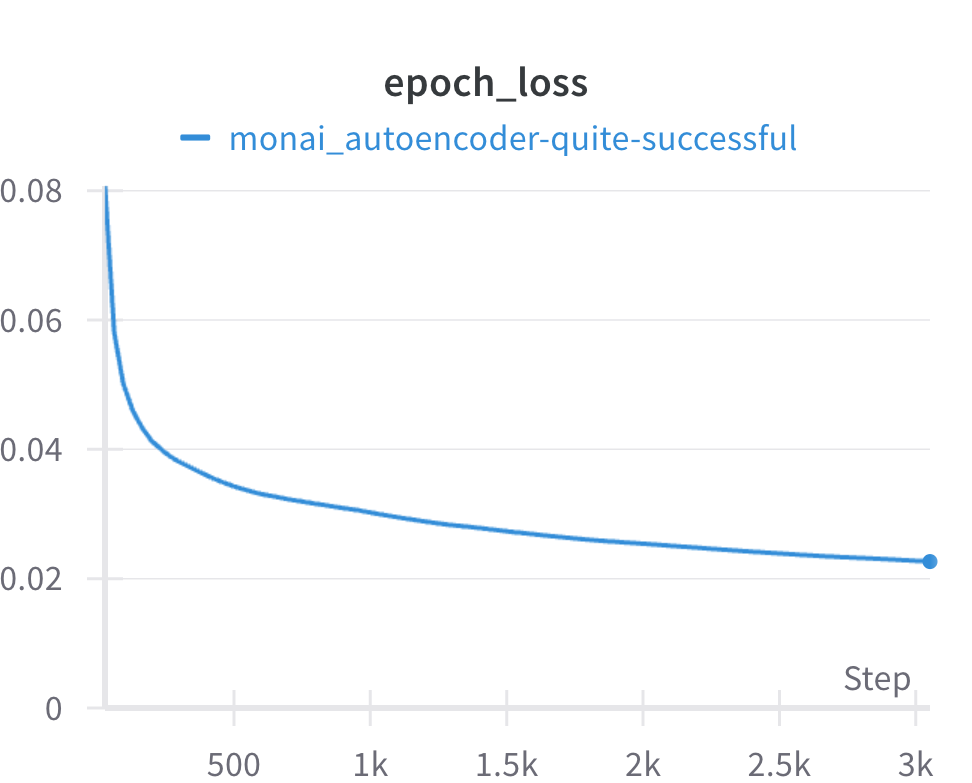
\includegraphics[width=\linewidth]{detailed_engineering/Monai Autoencoder/charts/epoch_loss.png}
\caption{}
\endminipage\hfill
\minipage{0.49\textwidth}
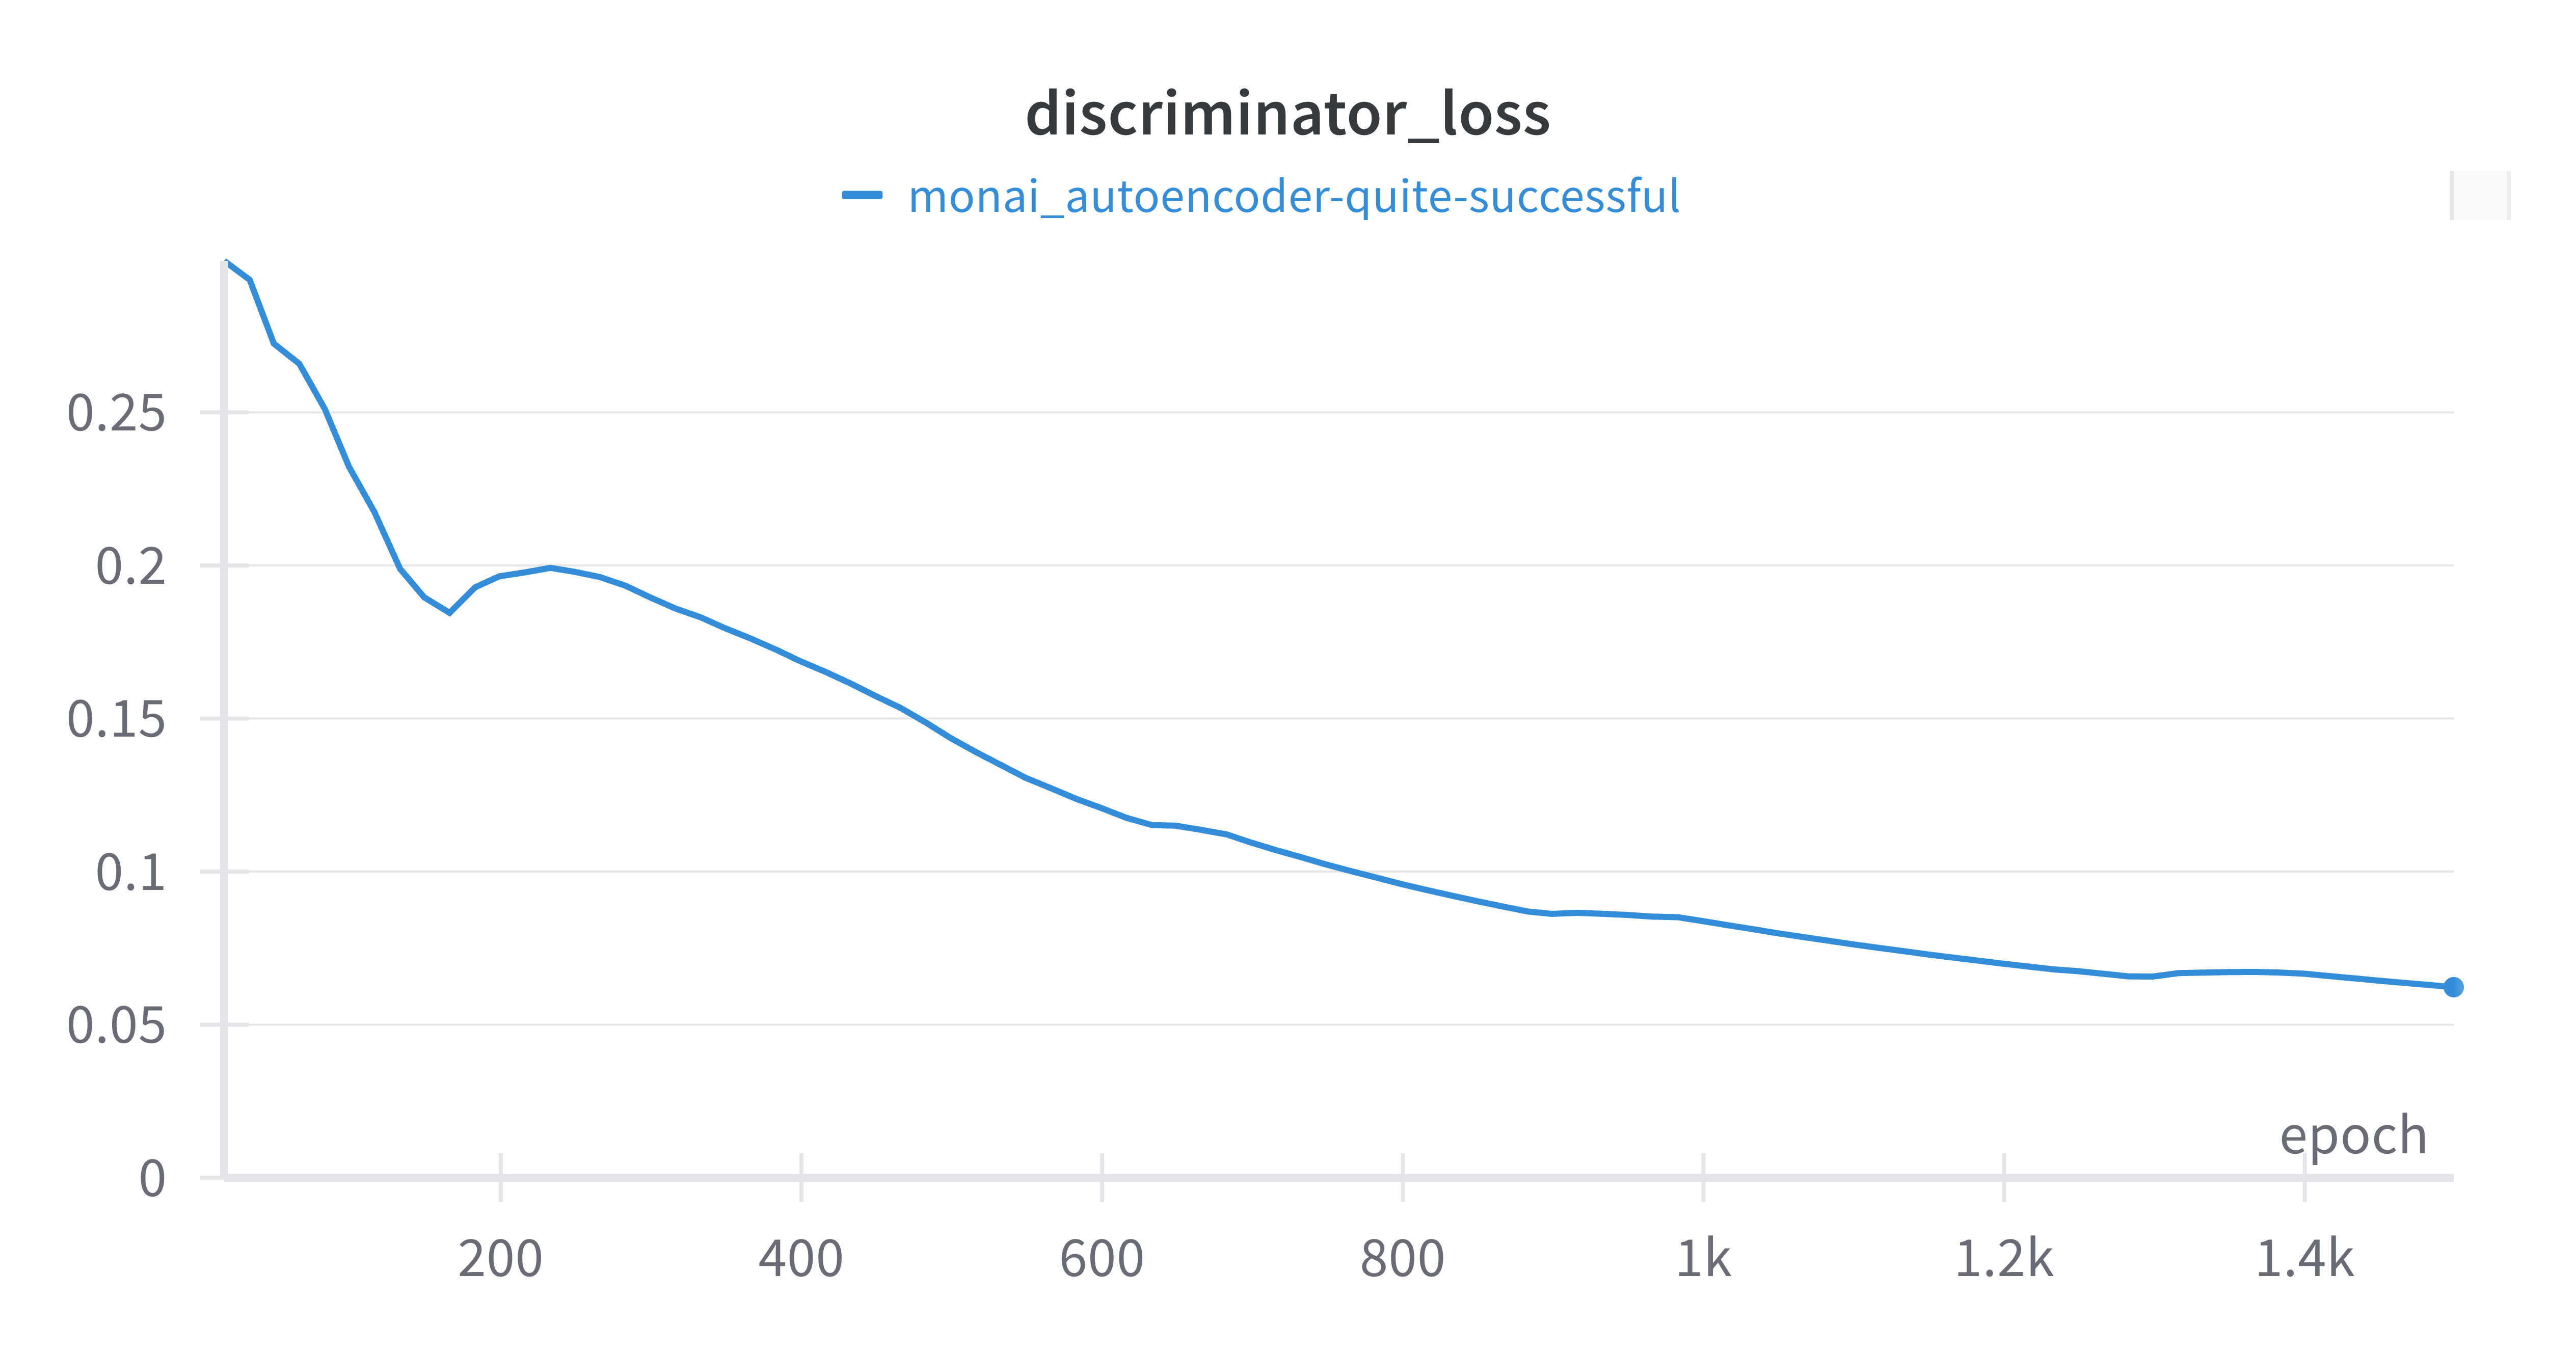
\includegraphics[width=\linewidth]{detailed_engineering/Monai Autoencoder/charts/discriminator_loss.png}
\caption{}
\endminipage
\end{figure}

\begin{figure}[H]
\minipage{0.49\textwidth}
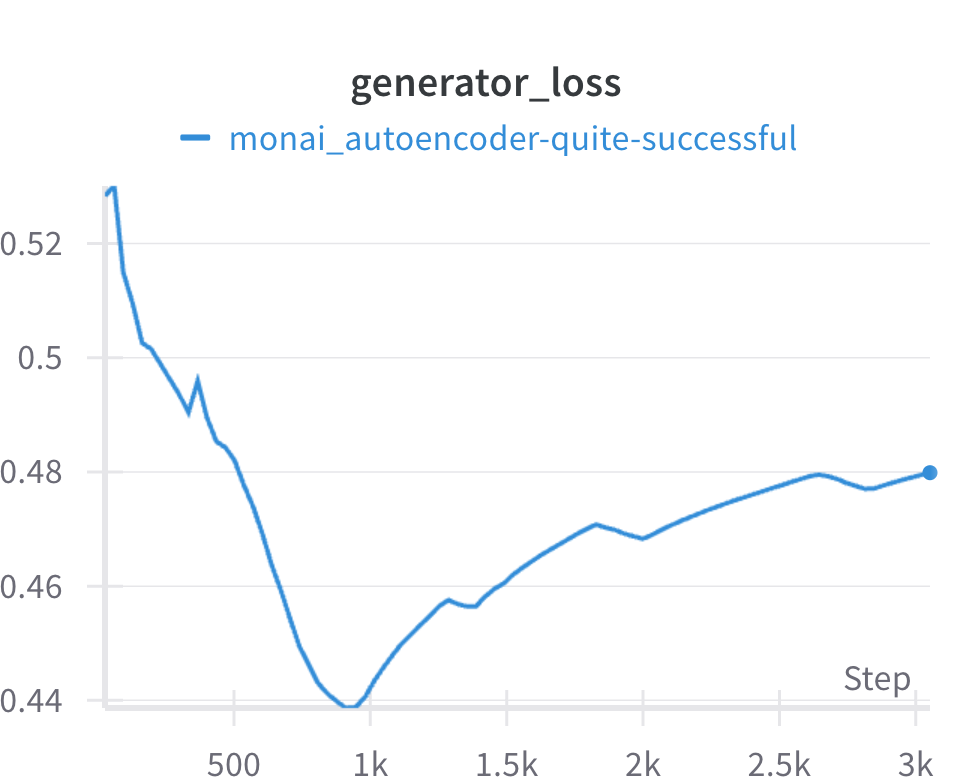
\includegraphics[width=\linewidth]{detailed_engineering/Monai Autoencoder/charts/generator_loss.png}
\caption{}
\endminipage\hfill
\minipage{0.49\textwidth}
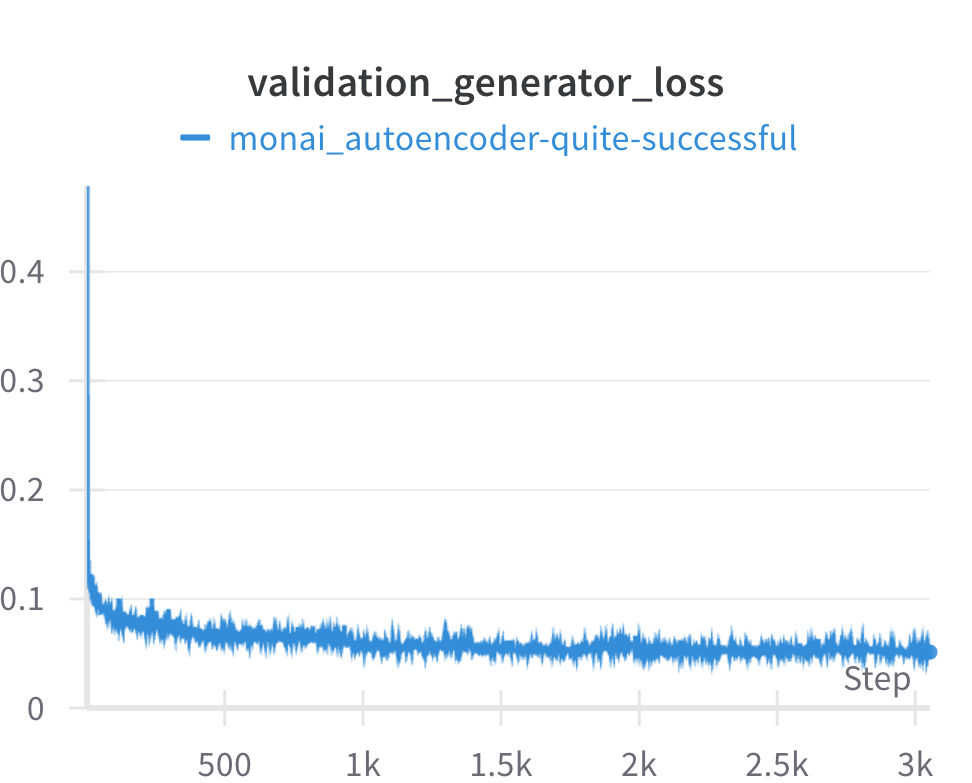
\includegraphics[width=\linewidth]{detailed_engineering/Monai Autoencoder/charts/val_generator_loss.png}
\caption{}
\endminipage
\end{figure}


\begin{figure}[H]
% \minipage{0.49\textwidth}
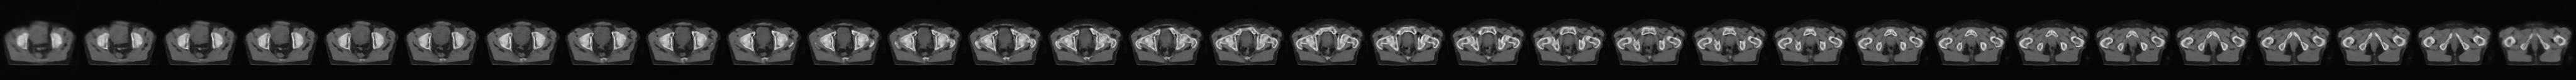
\includegraphics[width=\linewidth]{detailed_engineering/Monai Autoencoder/charts/reconstruction.png}
\caption{}
% \endminipage\hfill
% \minipage{0.49\textwidth}
% \includegraphics[width=\linewidth]{charts/Section-4-Panel-5-z2xepgyu7}
% \caption{}
% \endminipage
\end{figure}
d




\paragraph{LDM Attempt 1}\mbox{}\\

In this attempt $z$ was sampled from $\mathcal{N}(0,1)$ and passed through the decoder. 

\begin{figure}[H]
\minipage{0.49\textwidth}
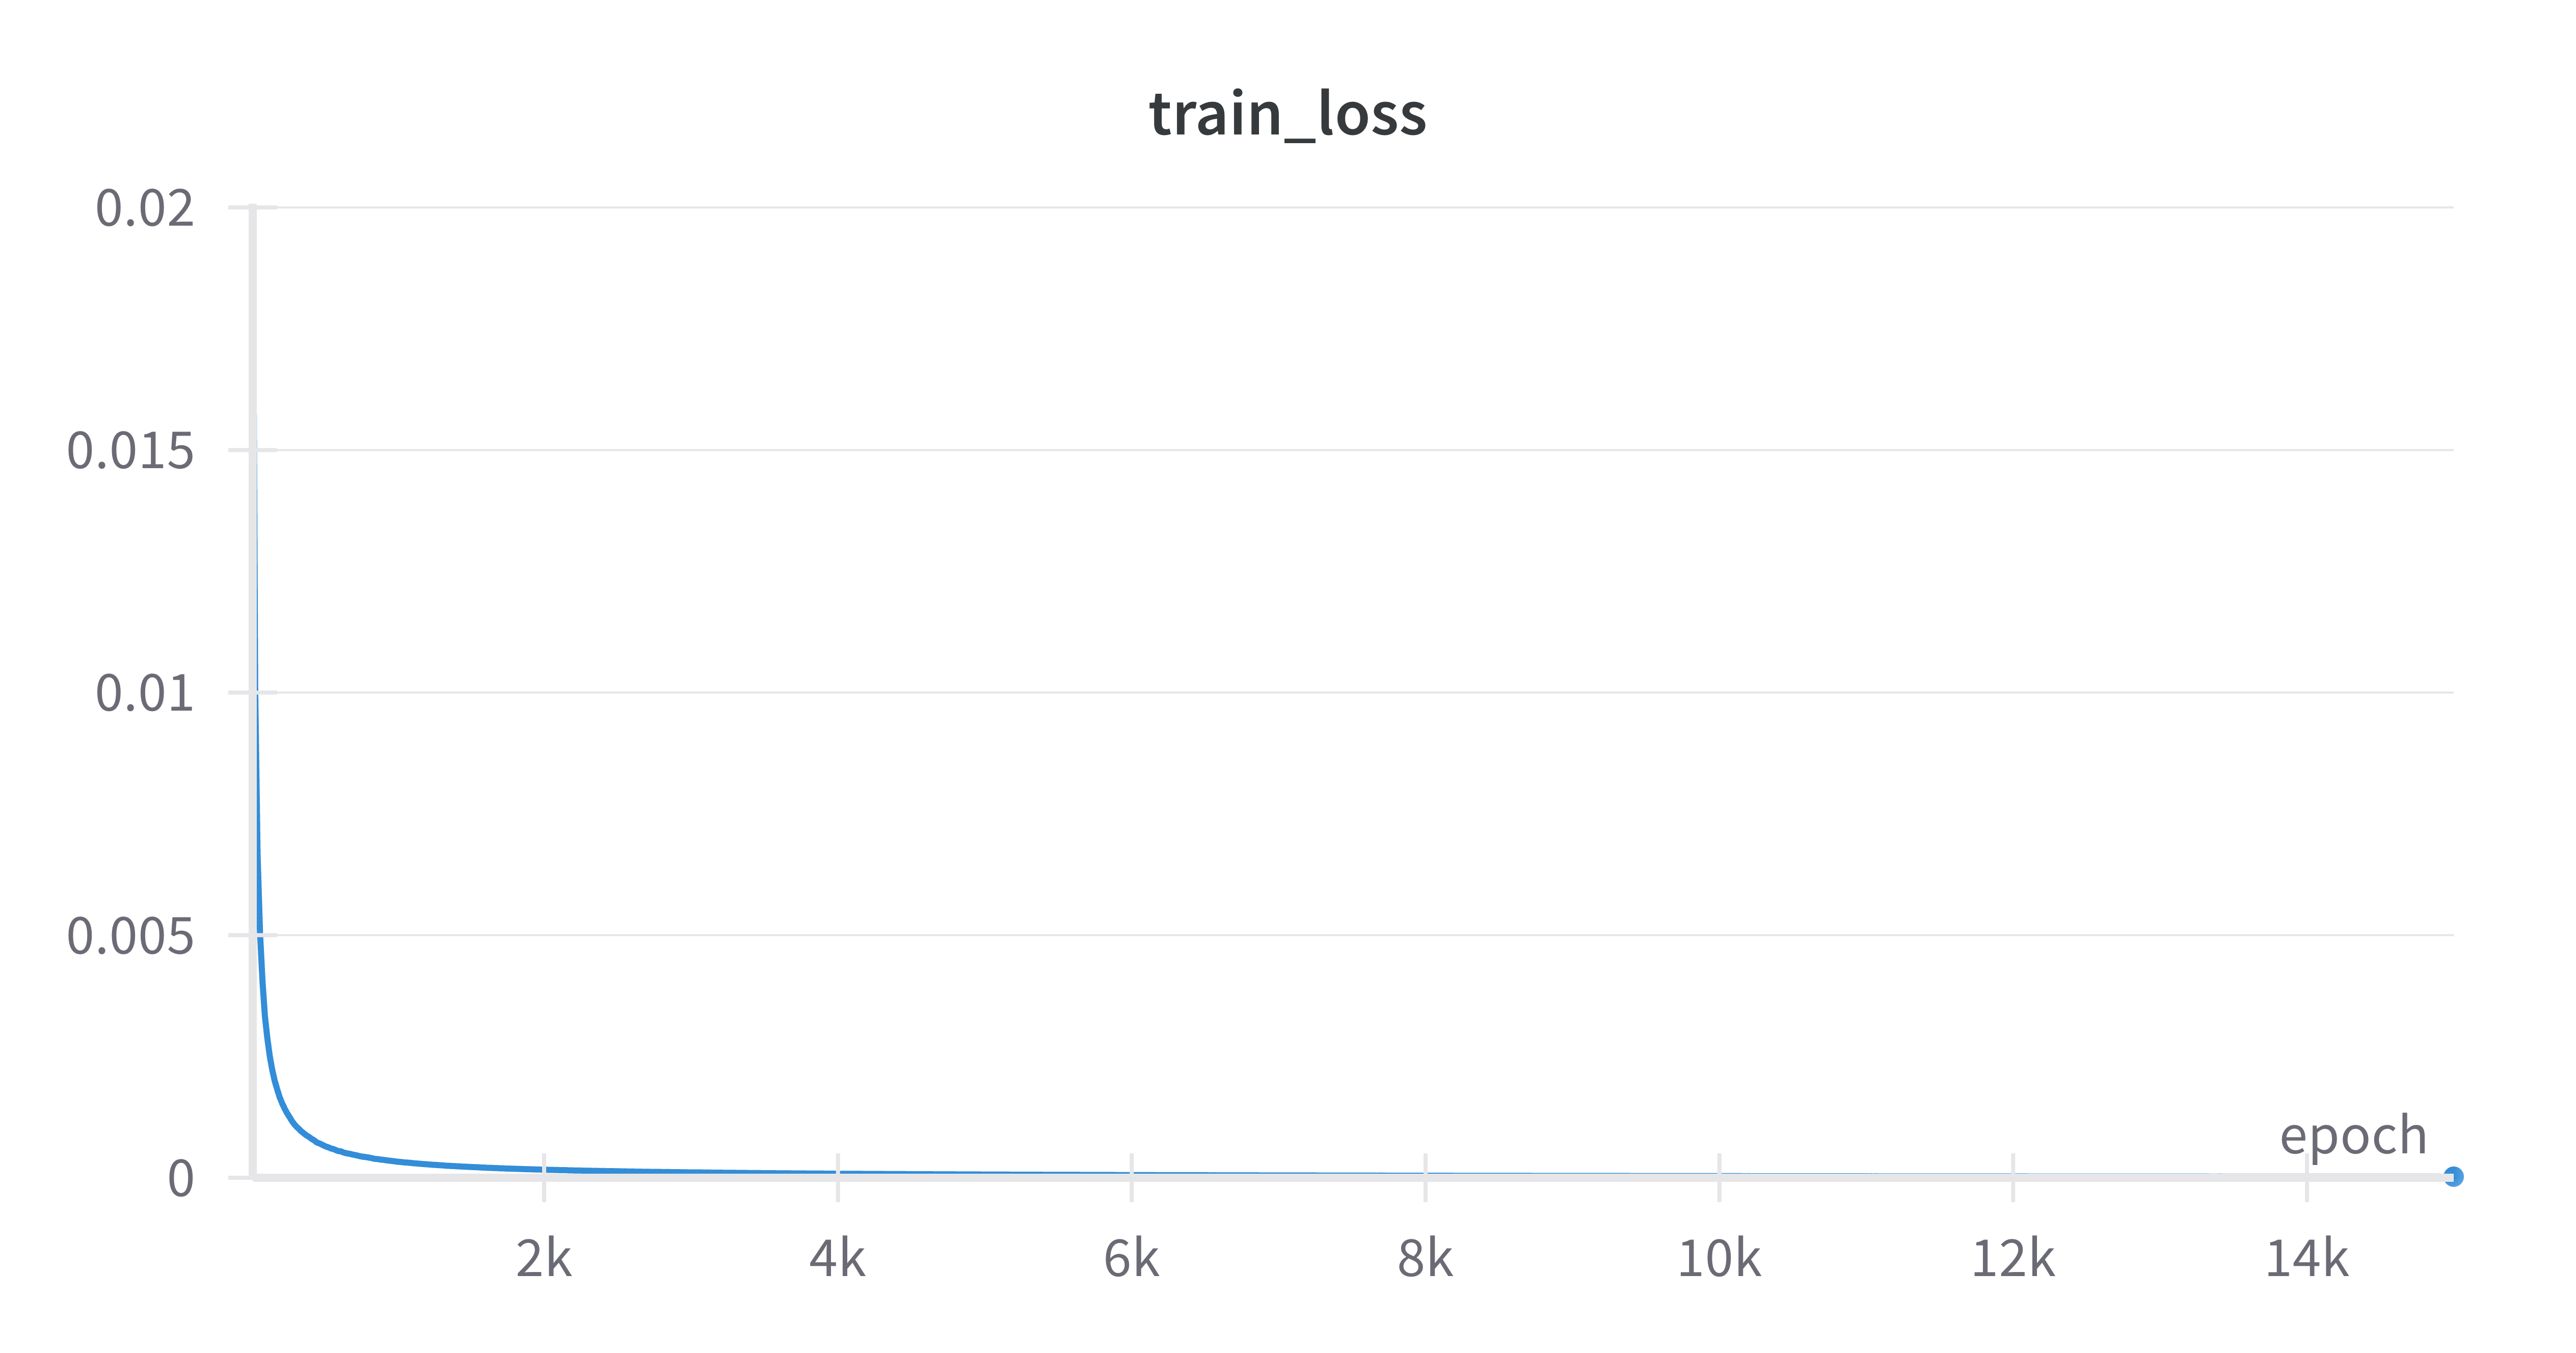
\includegraphics[width=\linewidth]{detailed_engineering/Monai Diffusion - Attempt 1/charts/train_loss.png}
\caption{}
\endminipage\hfill
\minipage{0.49\textwidth}
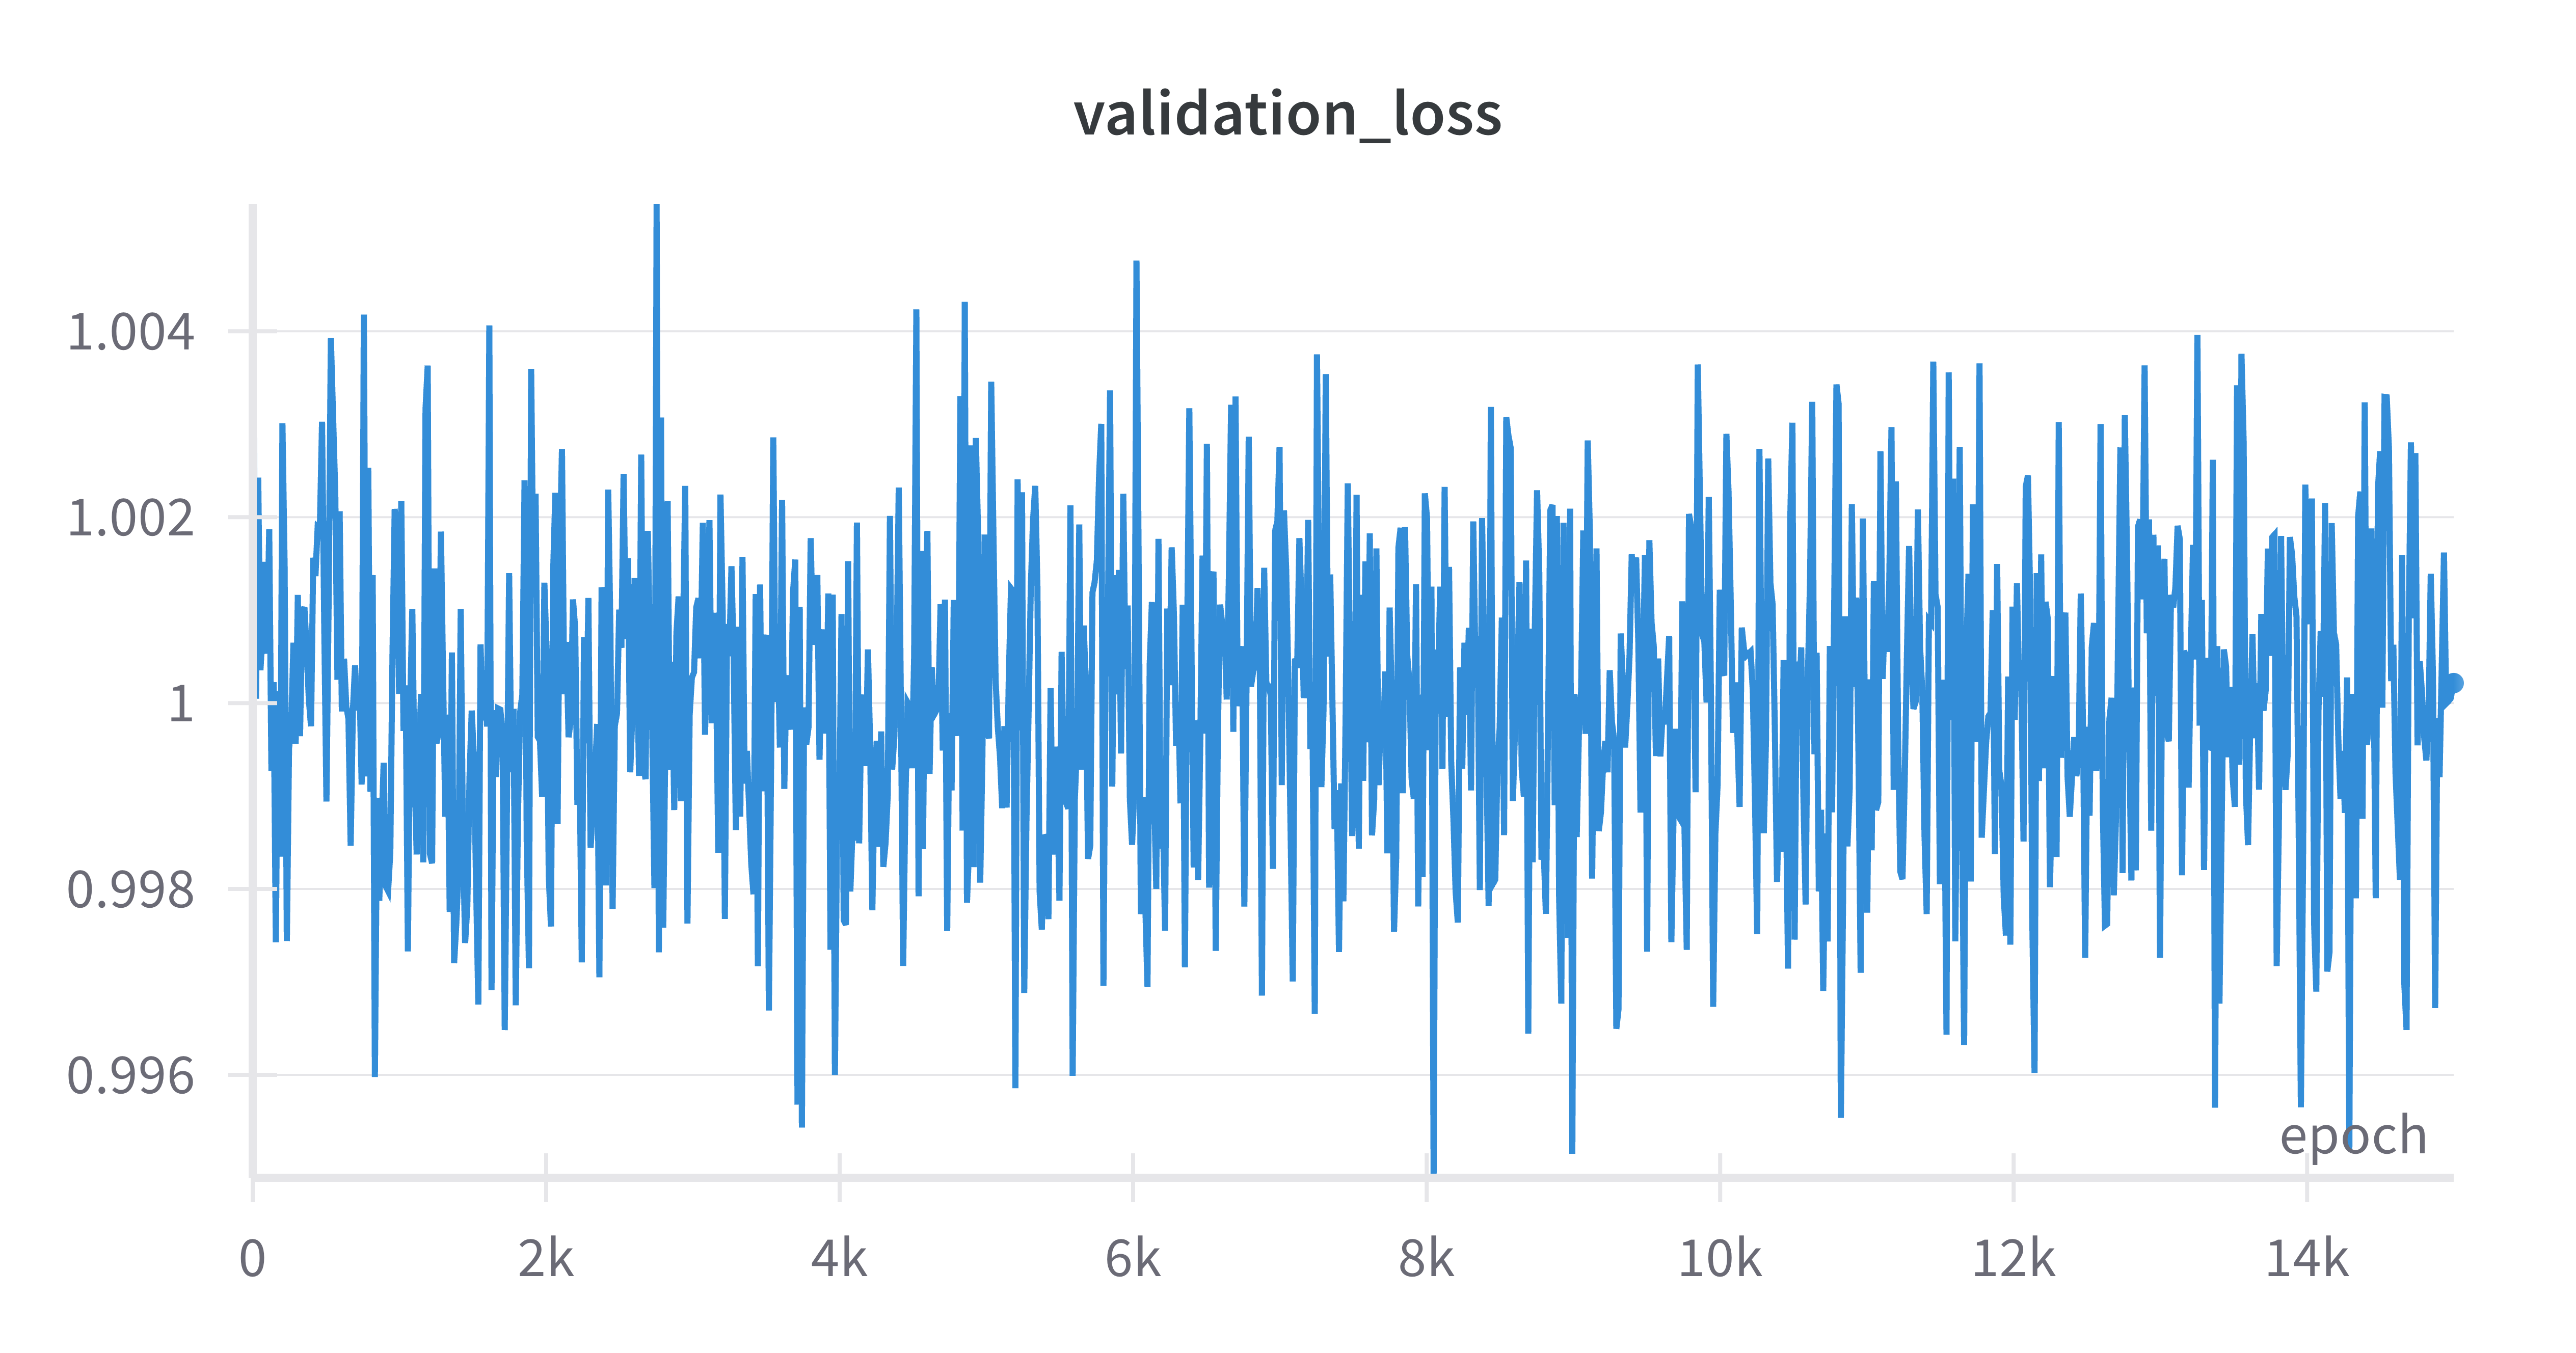
\includegraphics[width=\linewidth]{detailed_engineering/Monai Diffusion - Attempt 1/charts/validation_loss.png}
\caption{}
\label{fig:ldm_a1_val_loss}
\endminipage
\end{figure}


\begin{figure}[H]
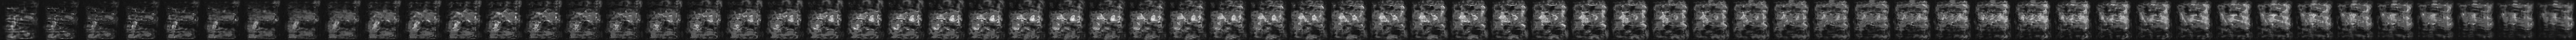
\includegraphics[width=\linewidth]{detailed_engineering/Monai Diffusion - Attempt 1/charts/generation.png}
\caption{Unsuccessful generation of synthetic CT scan.}
\label{fig:attempt1-generation}
\end{figure}

Generation was unsuccessful\ref{fig:attempt1-generation}. The validation loss did not decrease\ref{fig:ldm_a1_val_loss}.


\paragraph{LDM Attempt 2}\mbox{}\\

\indent In this attempt instead of creating noise from $\sim\mathcal{N}(0,1)$, the noise was generated from $N(\mu, \sigma)$ where $\mu$ is the mean of the training data $z_{\mu}$ and $\sigma$ is the mean of $z_{\sigma}$ obtained from the training data set (25 samples).

\paragraph{Model configuration}\mbox{}\\
The configuration was the same as in Attempt 1. The only difference was in the noise generation approach.

\paragraph{Training}\mbox{}\\
\begin{figure}[H]
\minipage{0.49\textwidth}
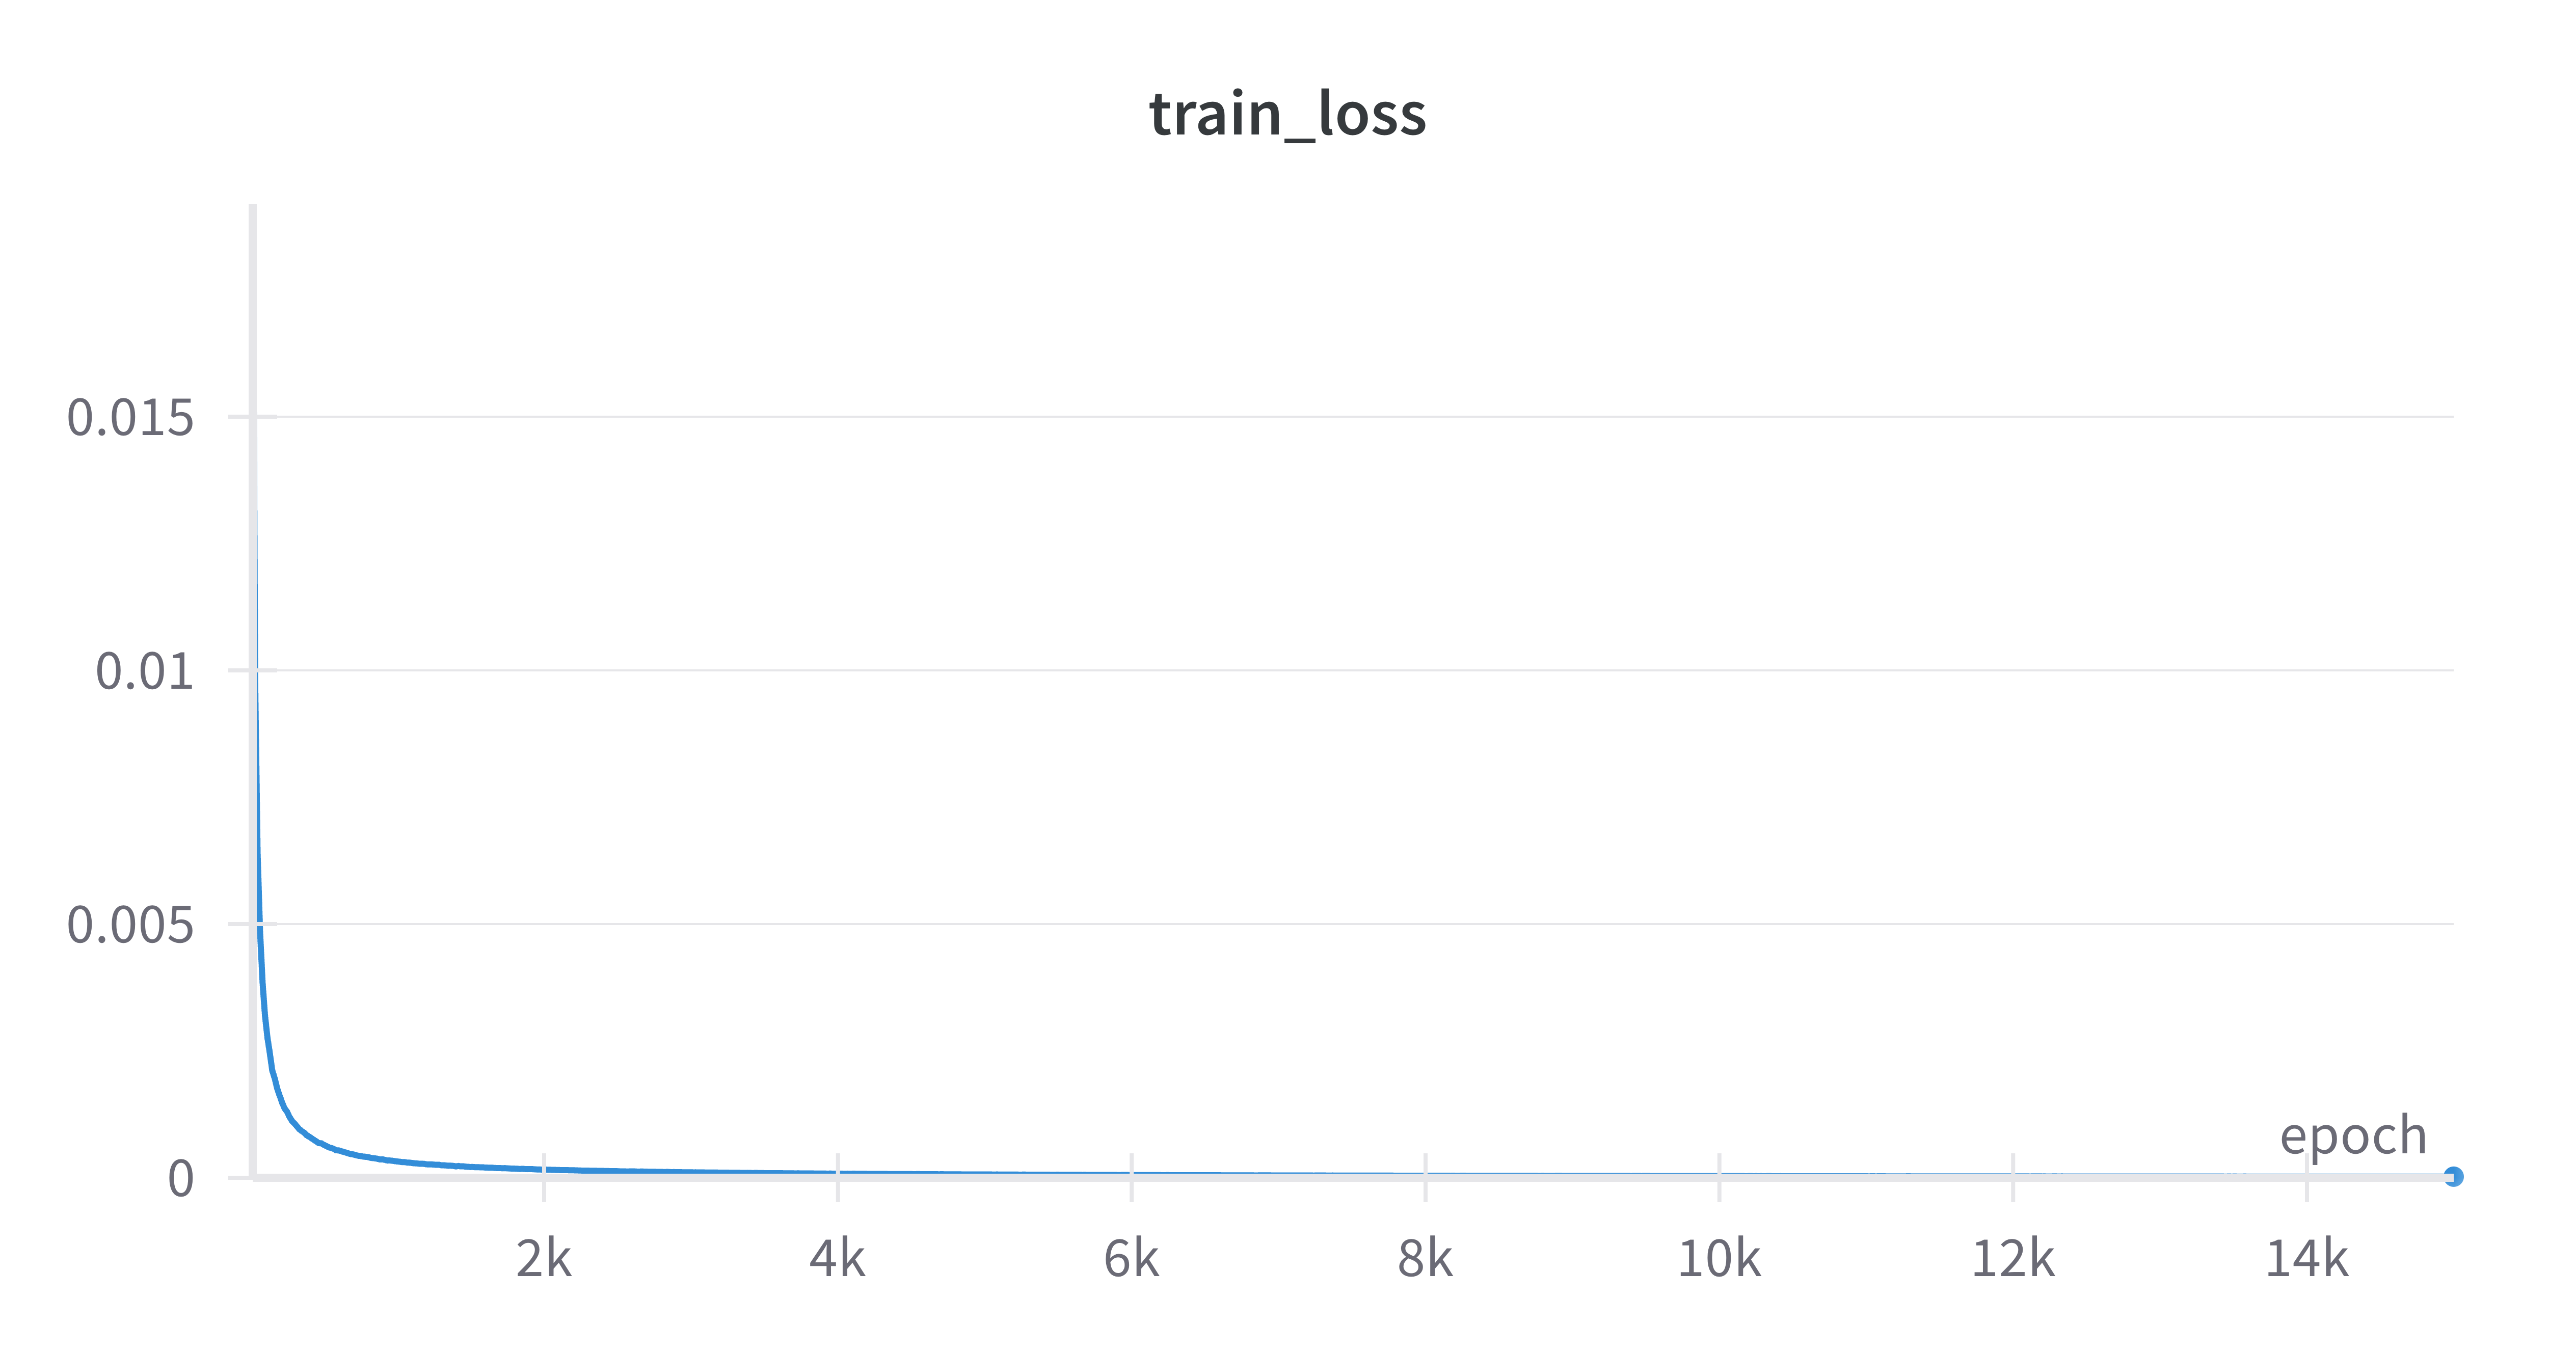
\includegraphics[width=\linewidth]{detailed_engineering/Monai Diffusion - Attempt 2/charts/train_loss.png}
\caption{}
\endminipage\hfill
\minipage{0.49\textwidth}
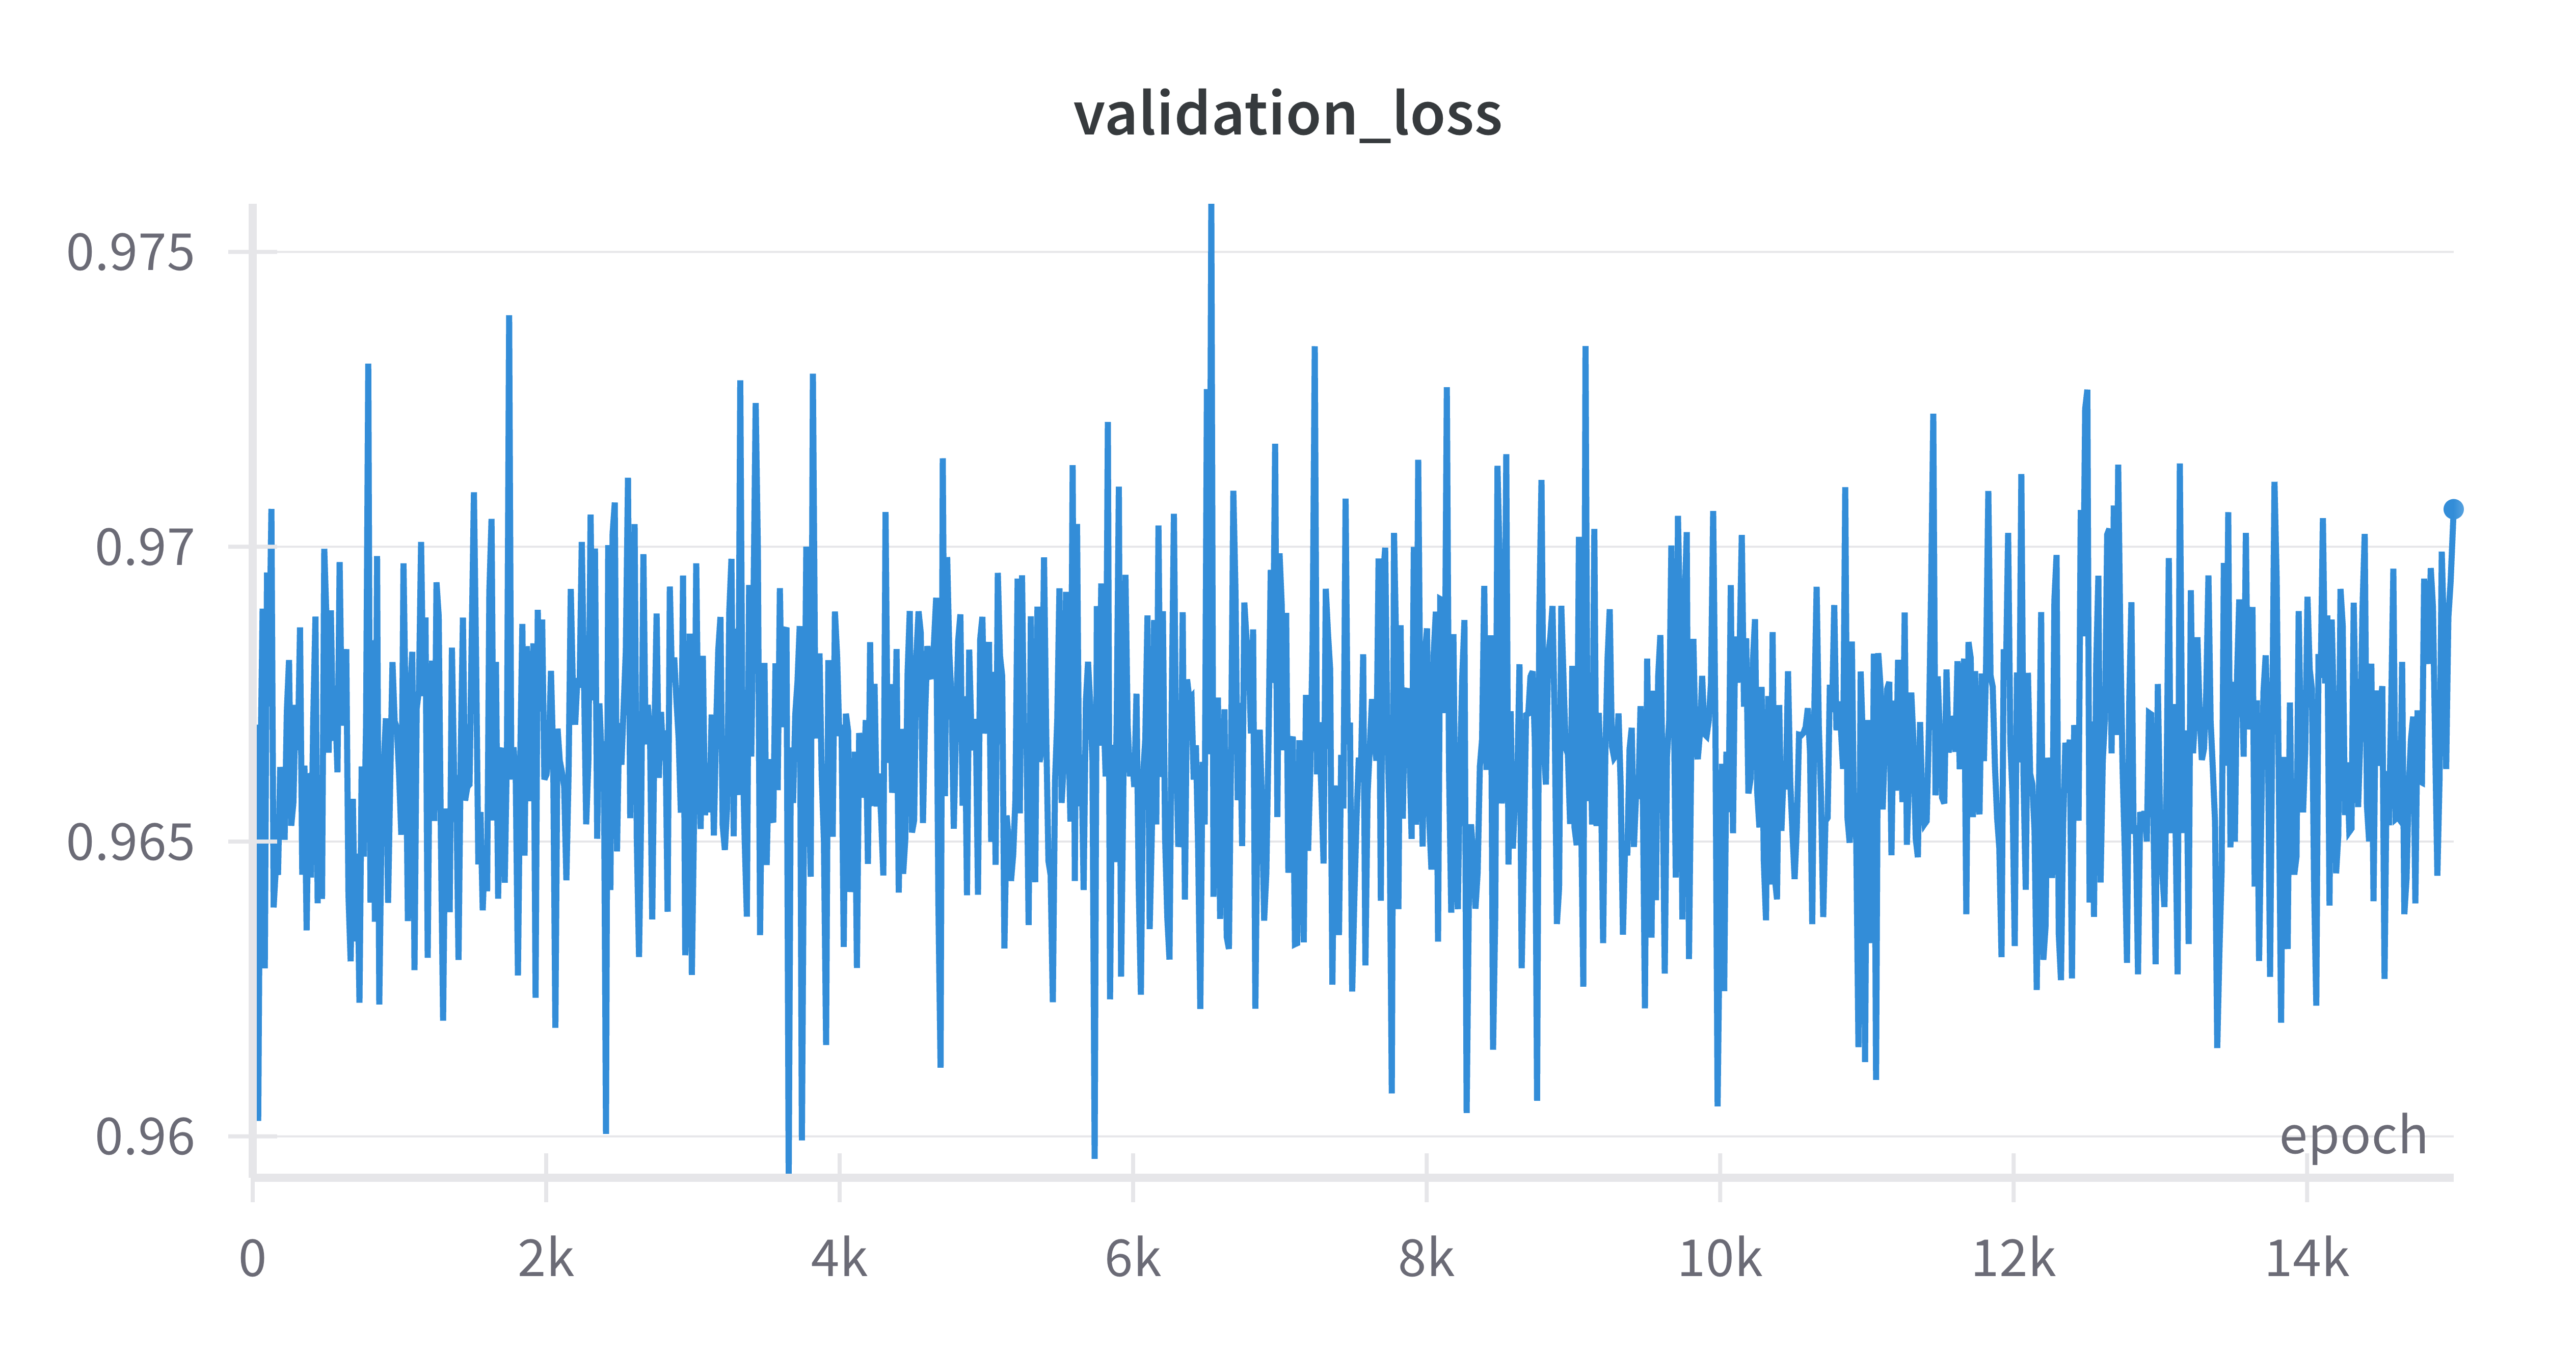
\includegraphics[width=\linewidth]{detailed_engineering/Monai Diffusion - Attempt 2/charts/validation_loss.png}
\caption{}
\label{fig:ldm_a2_val_loss}
\endminipage
\end{figure}

As is visible in the figure \ref{fig:ldm_a2_val_loss}, the validation loss did not decrease. The output of the generation was the same as in the previous attempt.






\newpage
\subsubsection{German VQVAE}
The VQVAE\footnote{\url{https://github.com/FirasGit/transformers_ct_reconstruction}} model and its complementation are based on the one presented in article\cite{khader_transformers_2023}.

Due to time constraints, the VQGAN and transformer models presented in the work have not been trained. Only VQVAE was trained and the result of this process is presented below. 


\paragraph{VQVAE}\mbox{}\\
\paragraph{Model configruation}\mbox{}\\

\begin{table}[h!]
\centering
\begin{tabular}{|l|l|}
\hline
\textbf{Parameter} & \textbf{Value} \\
\hline
\multicolumn{2}{|c|}{\textbf{Training}} \\
\hline
Accelerator & GPU \\
\hline
Devices & 2 \\
\hline
Precision & 32 \\
\hline
Strategy & DDP \\
\hline
Maximum Epochs & 10001 \\
\hline
\multicolumn{2}{|c|}{\textbf{Model}} \\
\hline
Input Channels & 1 \\
\hline
Output Channels & 1 \\
\hline
Embedding Channels & 8 \\
\hline
Number of Embeddings & 16384 \\
\hline
Spatial Dimensions & 3 \\
\hline
Hidden Channels & [32, 64, 128, 256] \\
\hline
Kernel Sizes & [3, 3, 3, 3] \\
\hline
Strides & [1, 2, 2, 2] \\
\hline
Embedding Loss Weight & 1 \\
\hline
Beta & 1 \\
\hline
Loss Function & L1 \\
\hline
Deep Supervision & 0 \\
\hline
Use Attention & [False, False, True, True] \\
\hline
Normalization & Group (num\_groups: 4, affine: True) \\
\hline
Sample Every N Epochs & 20 \\
\hline
Learning Rate & 5e-6 \\
\hline
\multicolumn{2}{|c|}{\textbf{Dataset}} \\
\hline
Caching & Disk \\
\hline
Path & /ravana/d3d\_work/micorl/data/ct\_images\_prostate\_32fixed/ \\
\hline
Image Size & 128 \\
\hline
Number of Slices & 32 \\
\hline
Window Width & 400 \\
\hline
Window Level & 60 \\
\hline
\end{tabular}
\caption{Parameters for the Training Configuration}
\label{table:training_params}
\end{table}

\paragraph{Training}\mbox{}\\

\begin{figure}[H]
\minipage{0.49\textwidth}
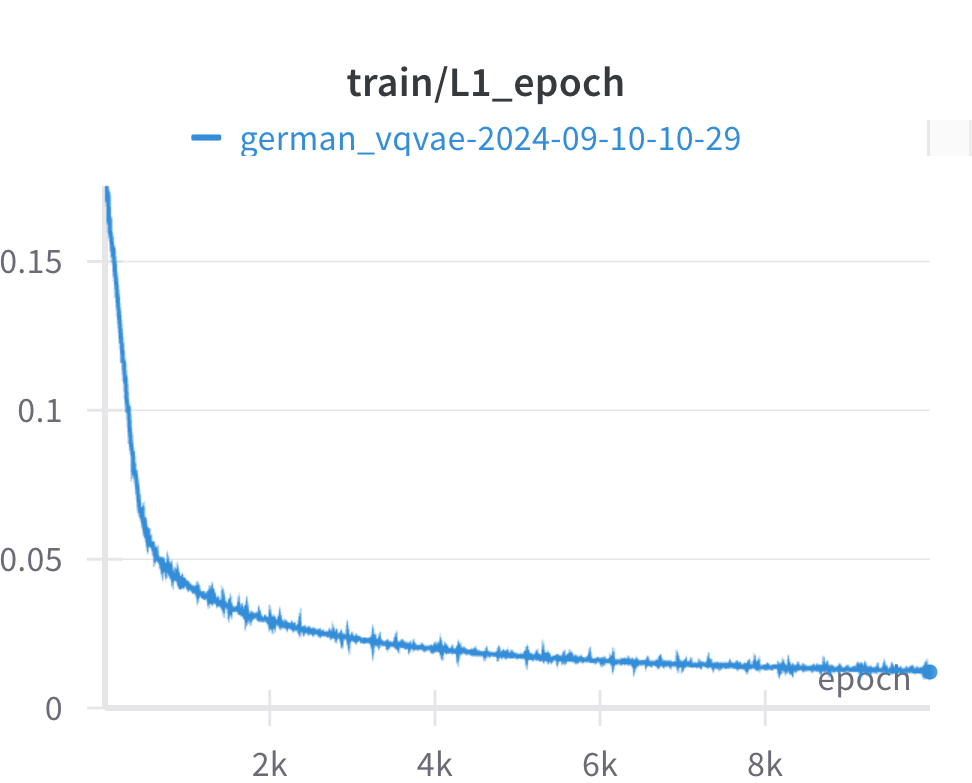
\includegraphics[width=\linewidth]{detailed_engineering/German VQVAE/charts/train_l1.png}
\caption{}
\endminipage\hfill
\minipage{0.49\textwidth}
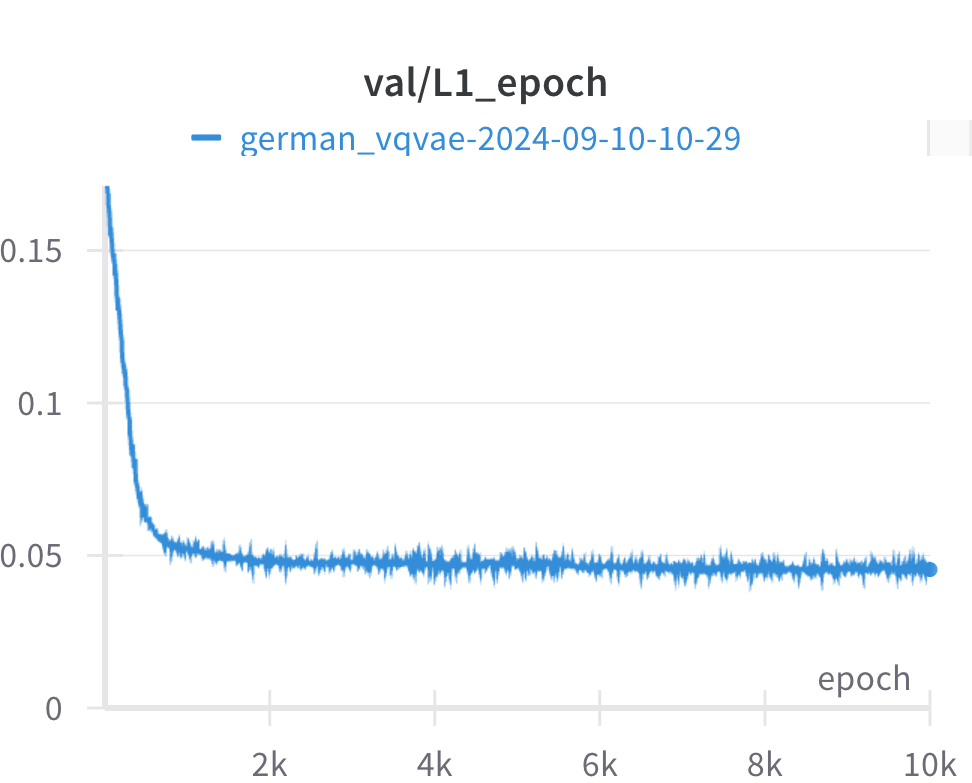
\includegraphics[width=\linewidth]{detailed_engineering/German VQVAE/charts/val_l1.png}
\caption{}
\endminipage
\end{figure}

\begin{figure}[H]
\minipage{0.49\textwidth}
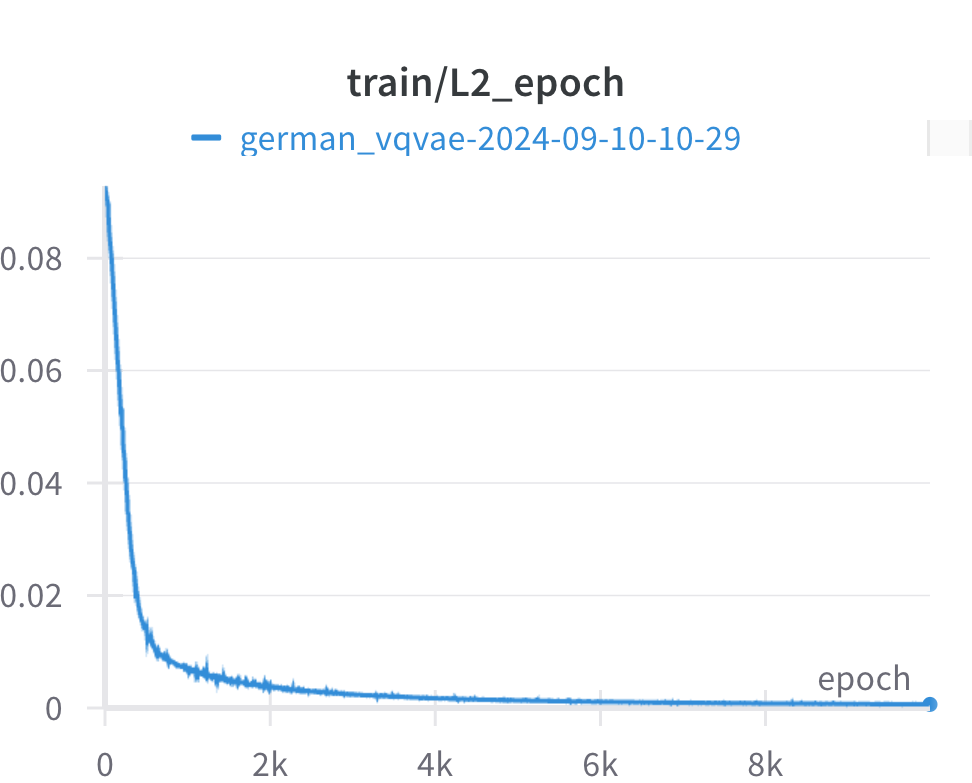
\includegraphics[width=\linewidth]{detailed_engineering/German VQVAE/charts/train_l2.png}
\caption{}
\endminipage\hfill
\minipage{0.49\textwidth}
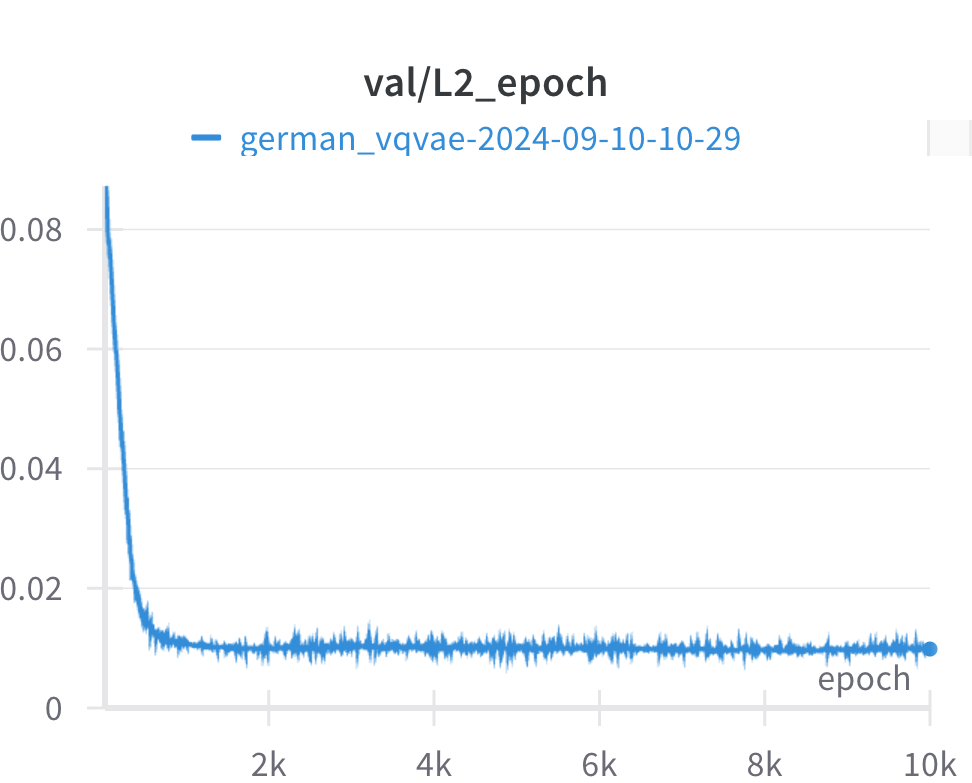
\includegraphics[width=\linewidth]{detailed_engineering/German VQVAE/charts/val_l2.png}
\caption{}
\endminipage
\end{figure}

\begin{figure}[H]
\minipage{0.49\textwidth}
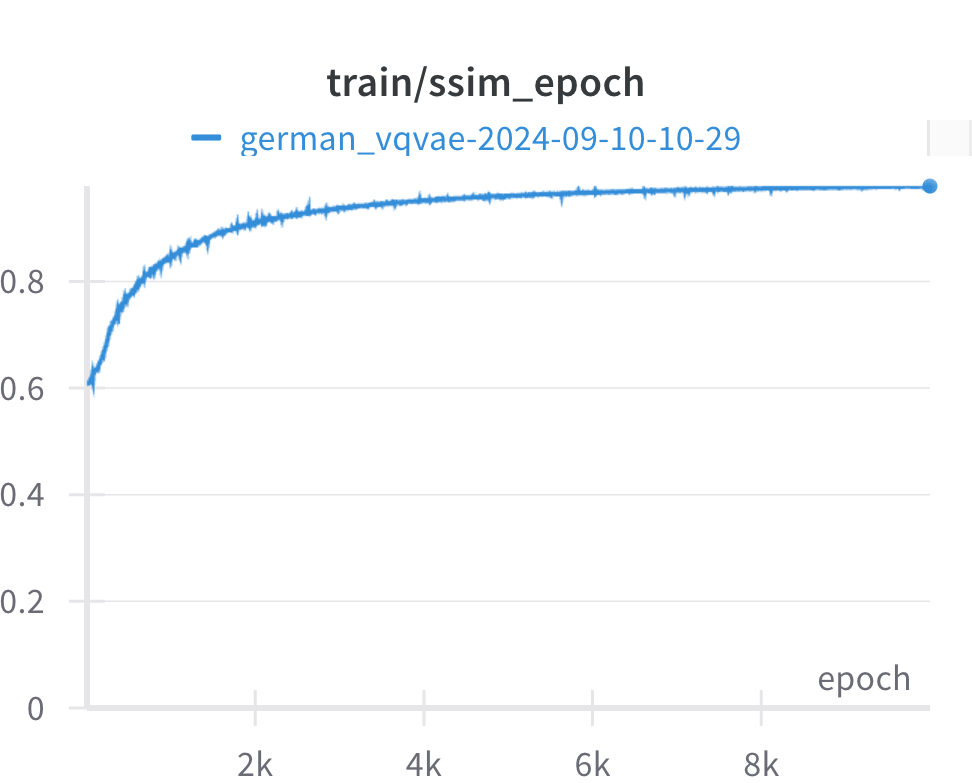
\includegraphics[width=\linewidth]{detailed_engineering/German VQVAE/charts/train_ssim.png}
\caption{}
\endminipage\hfill
\minipage{0.49\textwidth}
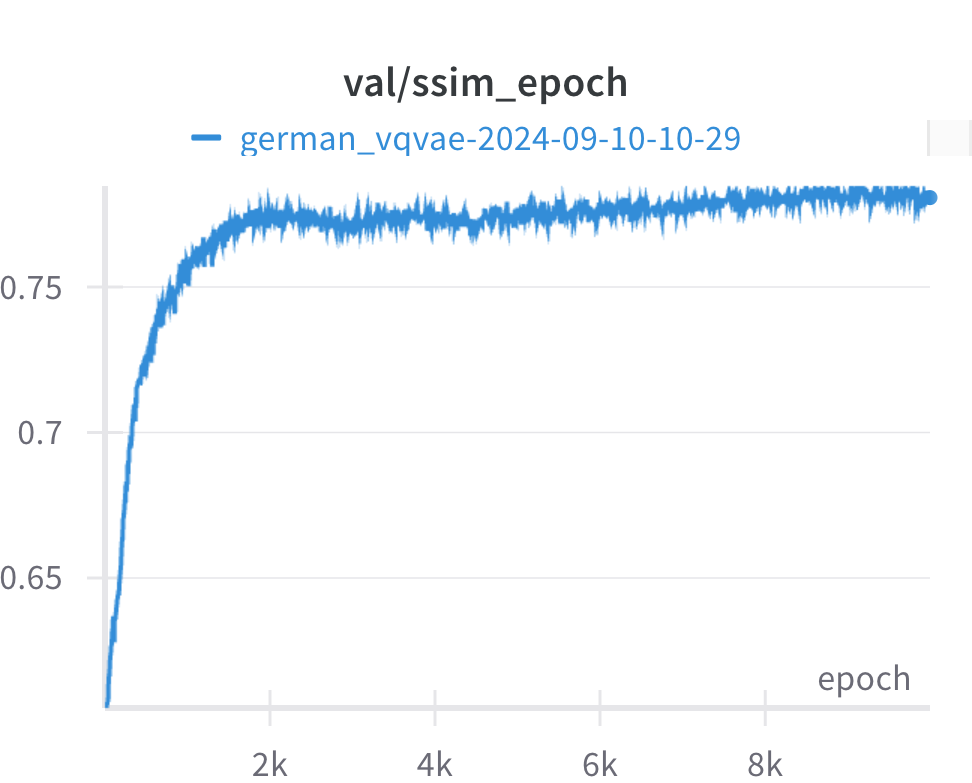
\includegraphics[width=\linewidth]{detailed_engineering/German VQVAE/charts/val_ssim.png}
\caption{}
\endminipage
\end{figure}




\paragraph{Results}\mbox{}\\

\begin{figure}[H]
    \centering
    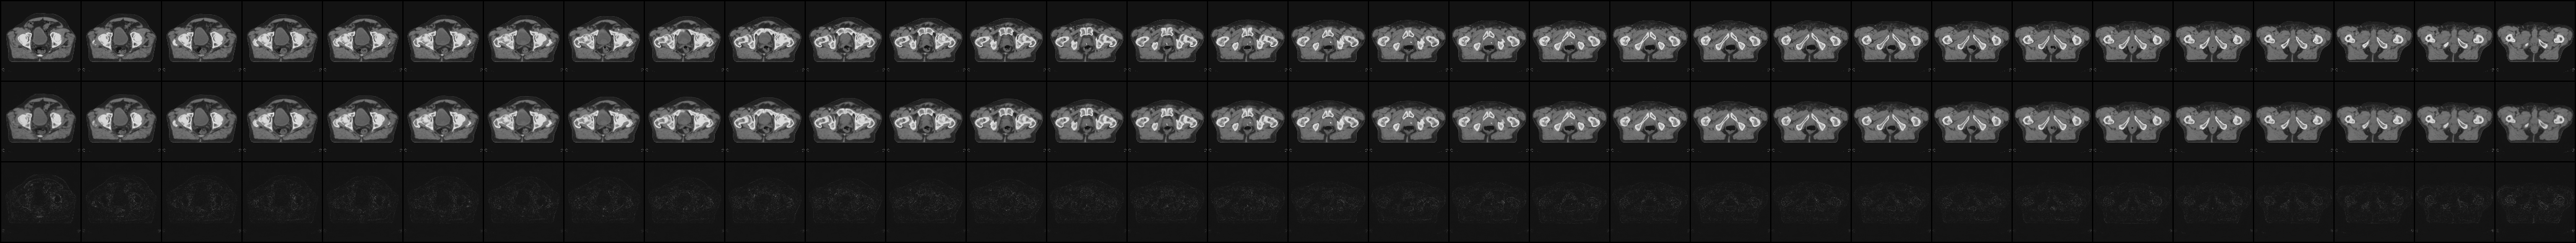
\includegraphics[width=\linewidth]{detailed_engineering/German VQVAE/charts/best_german_vqvae.png}
    \caption{The best quality reconstruction achieved. Epoch 8499, step 10540. Top - input, middle - reconstruction, bottom their difference}
    \label{fig:german_vqvae_best}
\end{figure}


\newpage
\subsubsection{Medical Diffusion VQGAN + DDPM}
\paragraph{Model configuration}

\paragraph{Training}
Objective: Minimize loss function defined as:

\begin{figure}[H]
\centering
\begin{subfigure}[h]{.45\linewidth}
    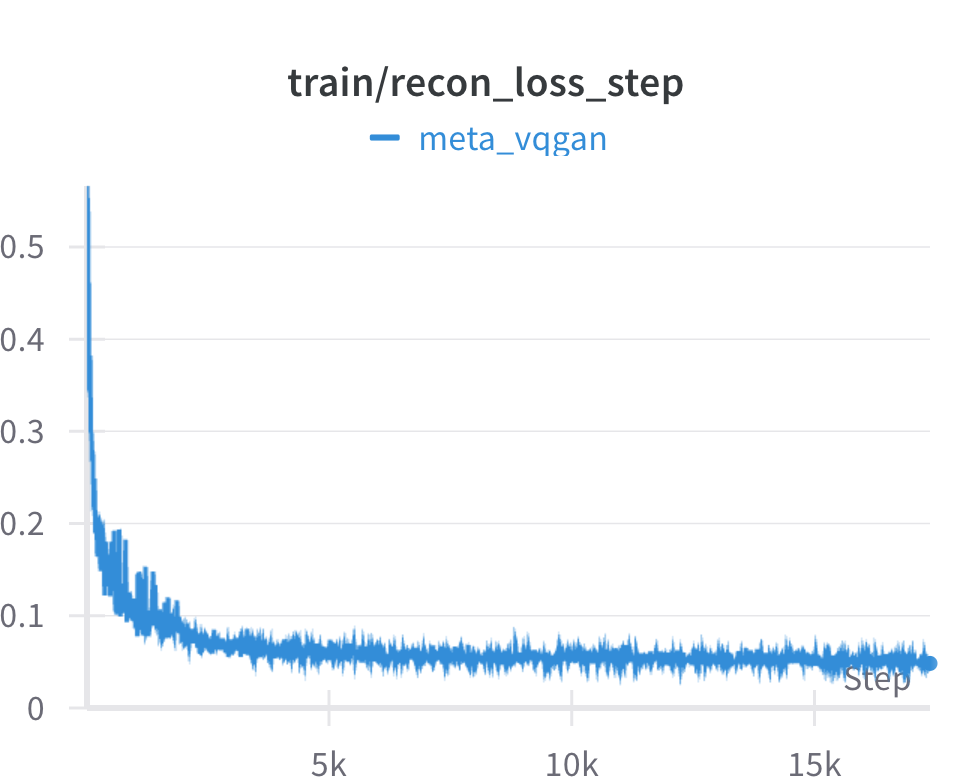
\includegraphics[width=\linewidth]{detailed_engineering/Meta VQGAN/charts/train_recon_loss_step.png}
    \caption{Caption}
    \label{fig:enter-label}
\end{subfigure}
\hfill
\begin{subfigure}[h]{.45\linewidth}
    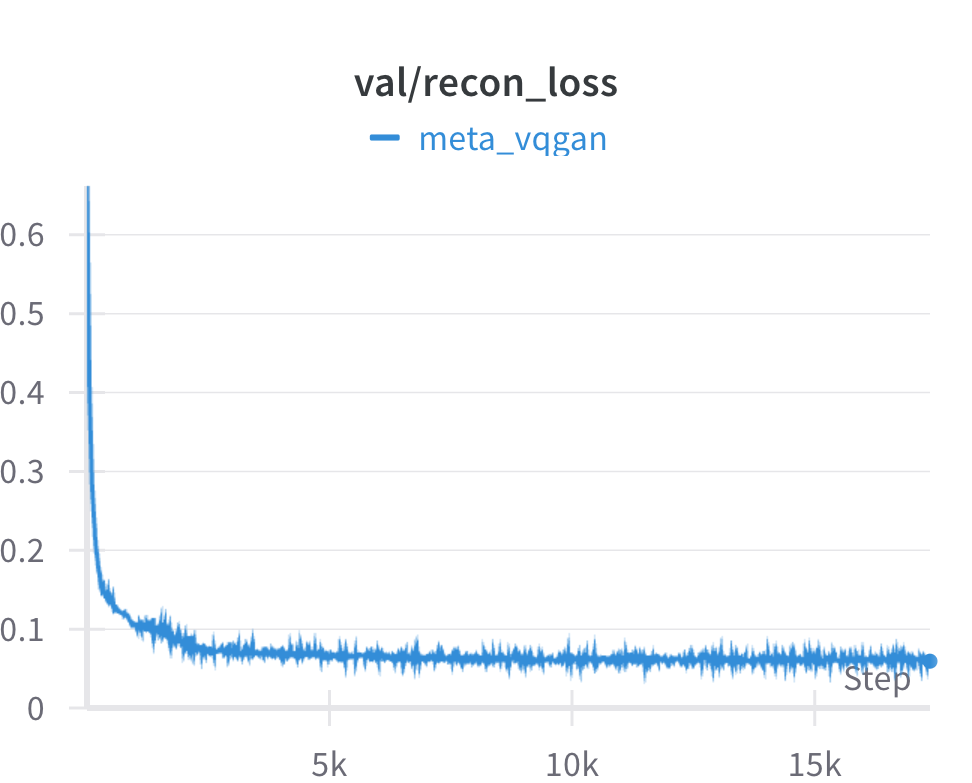
\includegraphics[width=\linewidth]{detailed_engineering/Meta VQGAN/charts/val_recon_loss.png}
    \caption{Caption}
    \label{fig:enter-label}
\end{subfigure}
\hfill
\begin{subfigure}[h]{.45\linewidth}
    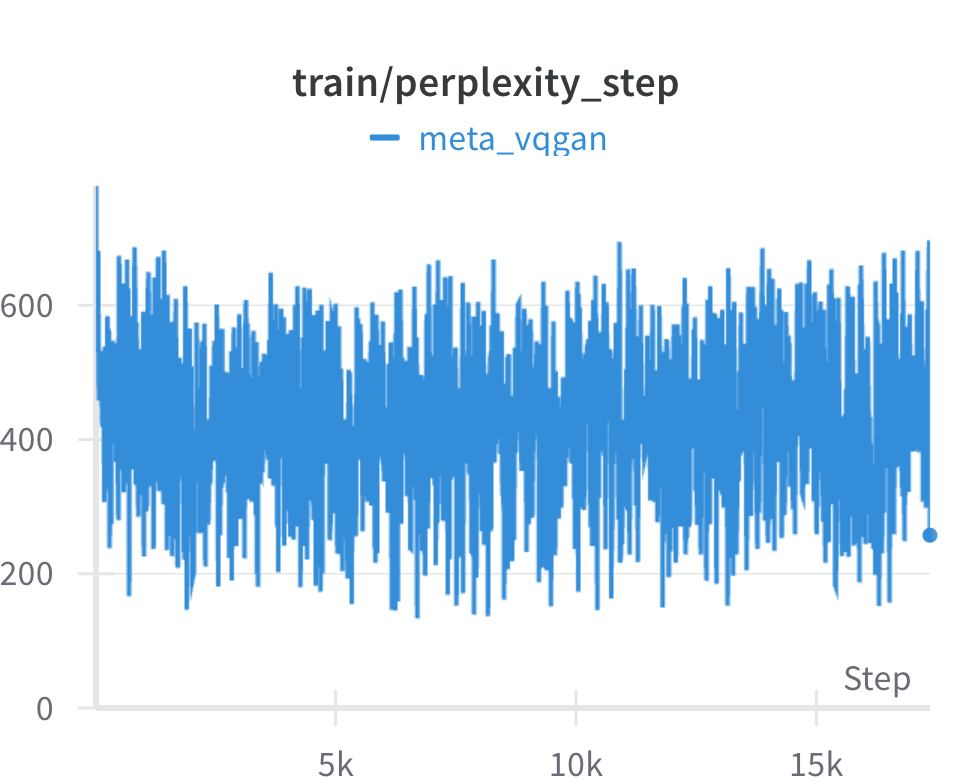
\includegraphics[width=\linewidth]{detailed_engineering/Meta VQGAN/charts/train_perplexity_step.png}
    \caption{Caption}
    \label{fig:enter-label}
\end{subfigure}
\hfill
\begin{subfigure}[h]{.45\linewidth}
    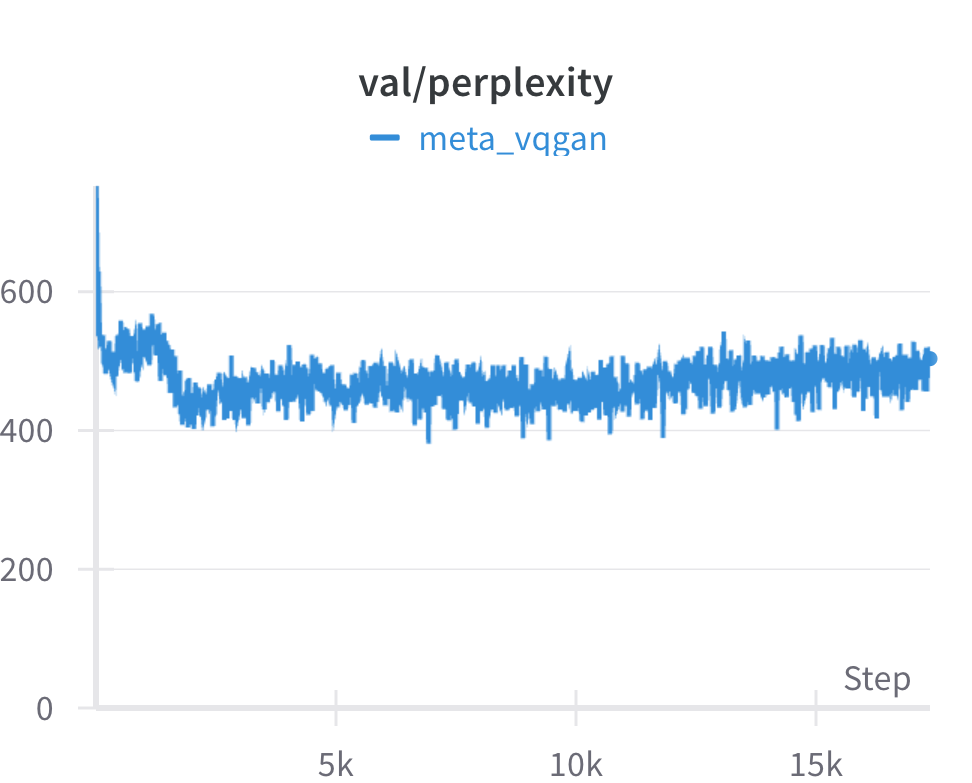
\includegraphics[width=\linewidth]{detailed_engineering/Meta VQGAN/charts/val_perplexity.png}
    \caption{Caption}
    \label{fig:enter-label}
\end{subfigure}
\hfill
\begin{subfigure}[h]{.45\linewidth}
    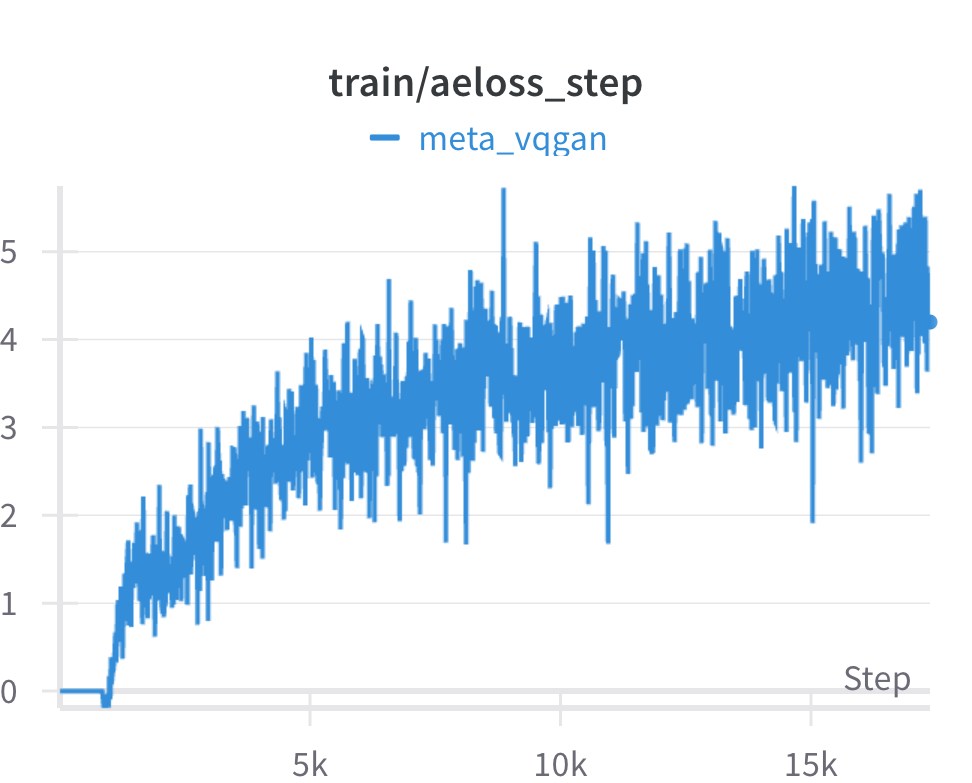
\includegraphics[width=\linewidth]{detailed_engineering/Meta VQGAN/charts/train_aeloss_step.png}
    \caption{Caption}
    \label{fig:enter-label}
\end{subfigure}
\hfill
\begin{subfigure}[h]{.45\linewidth}
    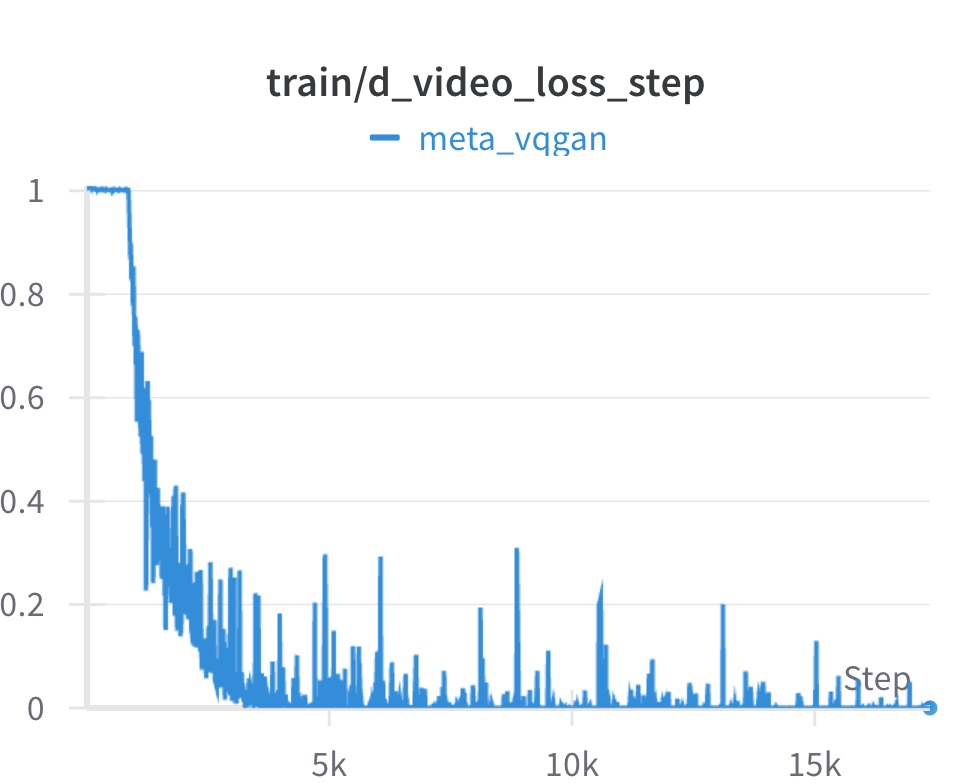
\includegraphics[width=\linewidth]{detailed_engineering/Meta VQGAN/charts/train_d_video_loss_step.png}
    \caption{Caption}
    \label{fig:enter-label}
\end{subfigure}
\hfill
% \begin{subfigure}[h]{.45\linewidth}
%     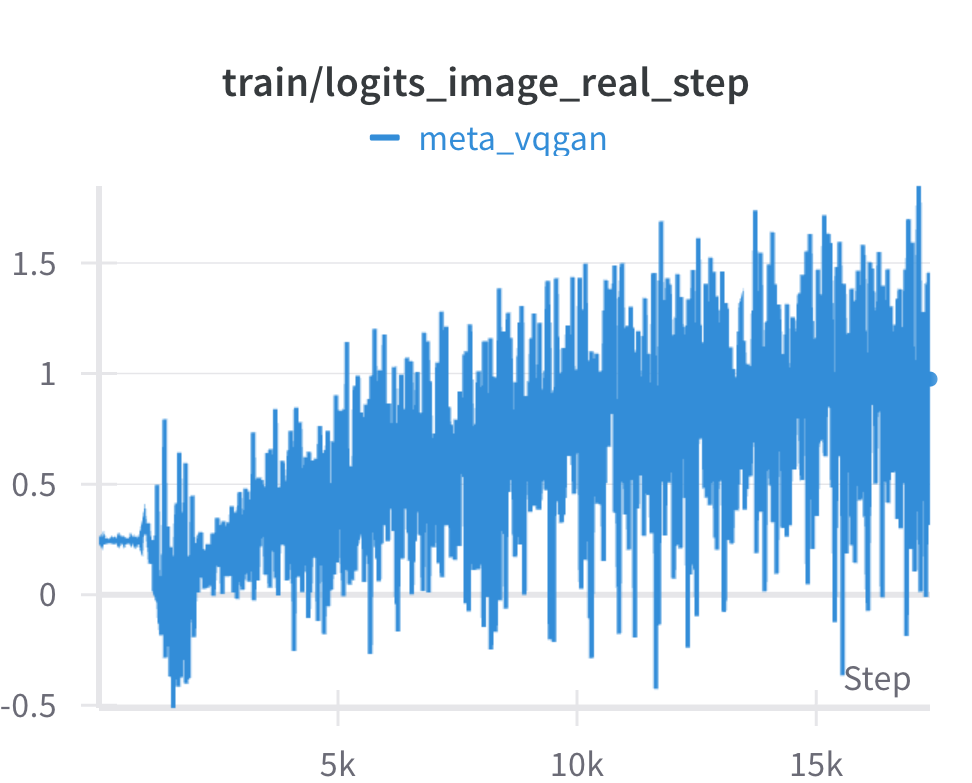
\includegraphics[width=\linewidth]{detailed_engineering/Meta VQGAN/charts/train_logits_image_real_step.png}
%     \caption{Caption}
%     \label{fig:enter-label}
% \end{subfigure}
% \hfill
% \begin{subfigure}[h]{.45\linewidth}
%     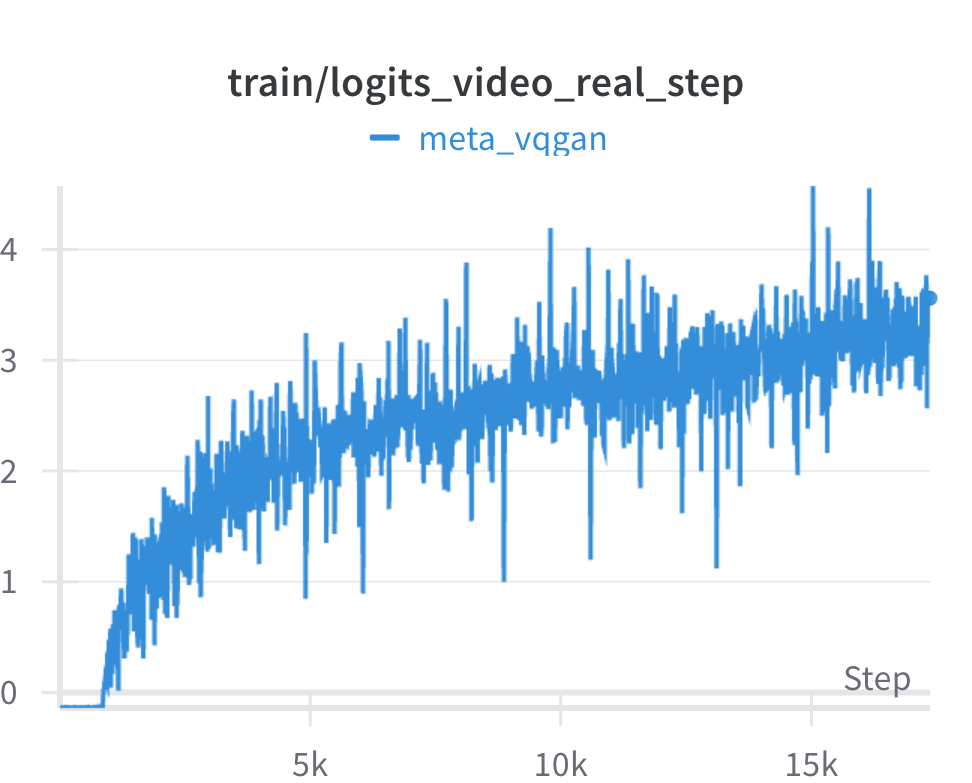
\includegraphics[width=\linewidth]{detailed_engineering/Meta VQGAN/charts/train_logits_video_real_step.png}
%     \caption{Caption}
%     \label{fig:enter-label}
% \end{subfigure}
\hfill
\begin{subfigure}[h]{.45\linewidth}
    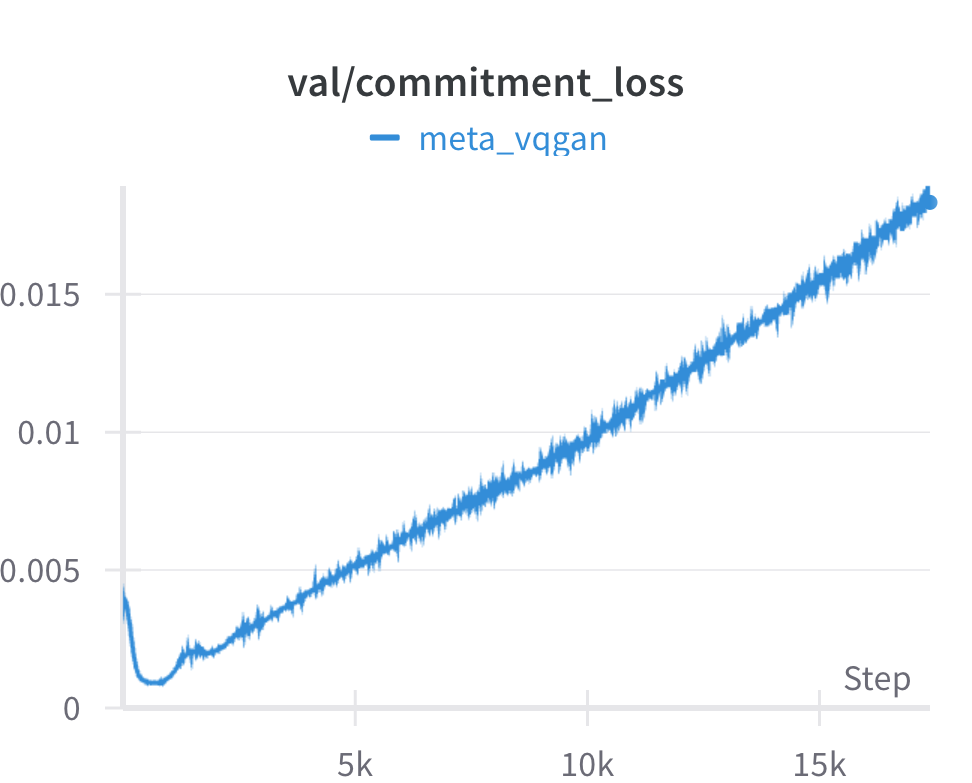
\includegraphics[width=\linewidth]{detailed_engineering/Meta VQGAN/charts/val_commitment_loss.png}
    \caption{Caption}
    \label{fig:enter-label}
\end{subfigure}
\hfill
\begin{subfigure}[h]{.45\linewidth}
    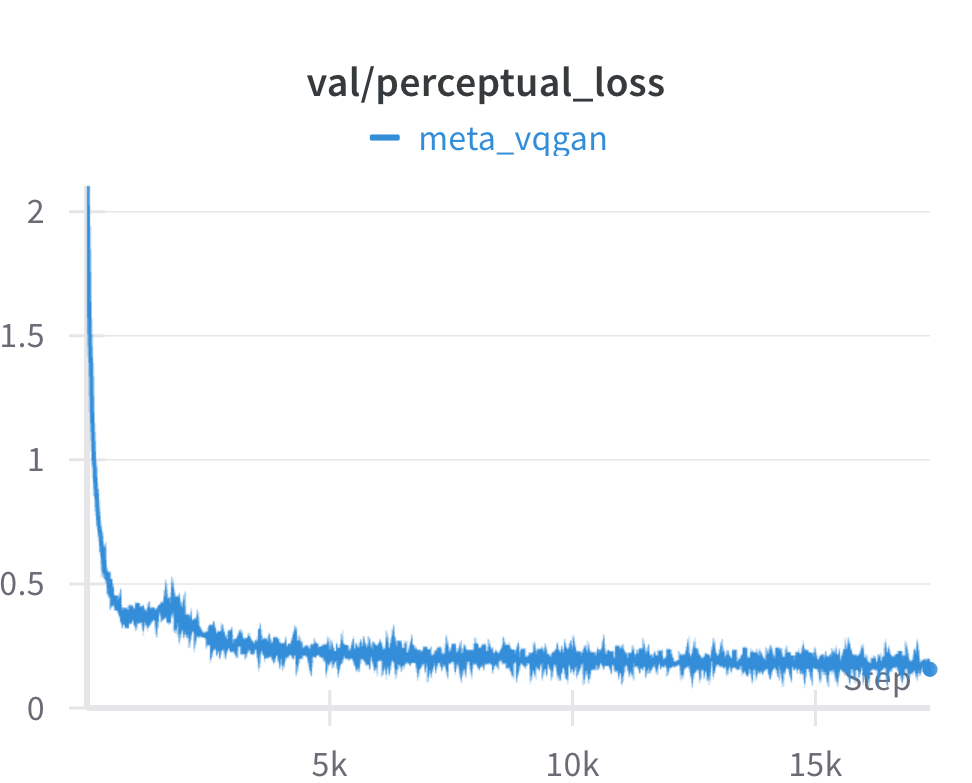
\includegraphics[width=\linewidth]{detailed_engineering/Meta VQGAN/charts/val_perceptual_loss.png}
    \caption{Caption}
    \label{fig:enter-label}
\end{subfigure}
\end{figure}


\paragraph{Results}

\newpage
\paragraph{Medical Diffusion DDPM}
\paragraph{Model configuration}

% \paragraph{Training}
% \begin{figure}[H]
% \centering
% \begin{subfigure}[h]{.45\linewidth}
%     \includegraphics[width=\linewidth]{detailed_engineering/}
%     \caption{Caption}
%     \label{fig:enter-label}
% \end{subfigure}
% \hfill
% \begin{subfigure}[h]{.45\linewidth}
%     \includegraphics[width=\linewidth]{detailed_engineering/Monai Autoencoder/charts/Section-4-Panel-2-bm1y05a9m.png}
%     \caption{Caption}
%     \label{fig:enter-label}
% \end{subfigure}
% \hfill
% \begin{subfigure}[h]{.45\linewidth}
%     \includegraphics[width=\linewidth]{detailed_engineering/Monai Autoencoder/charts/Section-4-Panel-3-dkwhik6ki.png}
%     \caption{Caption}
%     \label{fig:enter-label}
% \end{subfigure}
% \hfill
% \begin{subfigure}[h]{.45\linewidth}
%     \includegraphics[width=\linewidth]{detailed_engineering/Monai Autoencoder/charts/Section-4-Panel-4-d216pe2qa.png}
%     \caption{Caption}
%     \label{fig:enter-label}
% \end{subfigure}
% \hfill
% \begin{subfigure}[h]{.45\linewidth}
%     \includegraphics[width=\linewidth]{detailed_engineering/Monai Autoencoder/charts/Section-4-Panel-5-z2xepgyu7.png}
%     \caption{Caption}
%     \label{fig:enter-label}
% \end{subfigure}
% \end{figure}


\paragraph{Results}



% \input{monai}